\documentclass{amsart}

%\usepackage[notref,notcite]{showkeys}

%Put numbers to the left of ``Theorem'', etc.
\swapnumbers

% Symbol Packages
\usepackage{amssymb,empheq}
% For convenience
\usepackage{verbatim}
% Fonts
\usepackage[cal=euler,scr=rsfso]{mathalfa}
% Bib
\usepackage[alphabetic]{amsrefs}

% Hyperref
\usepackage{hyperref}

% TikZ settings
\usepackage{tikz}
\usetikzlibrary{matrix,arrows}


% Compile diagrams into seperate files.  (This is usually not worthwhile.)
%\CompileMatrices

\title[The Enriched Coherent Nerve]{Cartesian-Enriched Quasicategories and the Coherent Nerve}
\author[H. Gindi]{Harry Gindi}
\address{Department of Mathematics \\ University of Regensburg \\ Regensburg, Bavaria 93051}
\email{harry.gindi@gmail.com}
\date{\today}
\subjclass{ 18A30, 18B40, 18C10, 18C30, 18C35, 18D05,
18D50, 18E35, 18G50, 18G55, 55P10, 55P15, 55Q05, 55U35, 55U40}
\keywords{enriched categories, higher category theory}


% For temporary questions.  For example, \margnote{This is something
% I'm confused about.} puts that message in the margin.
\newcommand{\margnote}[1]{\mbox{}\marginpar{\tiny\hspace{0pt}#1}}



% To get ``linear'' numbering of subsections and theorems.
\numberwithin{equation}{section}

% why does this work?
\makeatletter
  \let\c@subsection\c@equation
\makeatother

\theoremstyle{plain}   %% This is the default, anyway

% Standard theorem types.
\newtheorem{thm}[subsection]{Theorem}
\newtheorem{prop}[subsection]{Proposition}
\newtheorem{cor}[subsection]{Corollary}
\newtheorem{lemma}[subsection]{Lemma}
\newtheorem{claim}[subsection]{Claim}
\newtheorem{conjecture}[subsection]{Conjecture}

\theoremstyle{remark}
\newtheorem{rem}[subsection]{Remark}    
\newtheorem{note}[subsection]{Note}   
\newtheorem{example}[subsection]{Example}
\newtheorem{ques}[subsection]{Question}
\newtheorem{defn}[subsection]{Definition}
\newtheorem{exer}[subsection]{Exercise}
\newtheorem{warning}[subsection]{Warning}
\renewcommand{\therem}{}

\theoremstyle{plain}


%%% standard operators for mathematics

% general categorical things
\DeclareMathOperator{\id}{id}
\DeclareMathOperator{\Sp}{Sp}
\DeclareMathOperator{\Sc}{Sc}
\DeclareMathOperator{\Sd}{Sd}
\DeclareMathOperator{\Pb}{Pb}
\DeclareMathOperator{\colim}{colim}
\DeclareMathOperator*{\coliml}{colim}
\DeclareMathOperator{\limw}{lim}
\DeclareMathOperator{\Cok}{Cok}
\DeclareMathOperator{\cok}{cok}
\DeclareMathOperator{\Ker}{Ker}
\DeclareMathOperator{\im}{im}
\DeclareMathOperator{\Ob}{Ob}
\DeclareMathOperator{\El}{El}
\DeclareMathOperator{\Psh}{Psh}
\DeclareMathOperator{\ob}{ob}
\DeclareMathOperator{\Aut}{Aut}
\DeclareMathOperator{\End}{End}
\DeclareMathOperator{\Lan}{Lan}
\newcommand{\op}{\ensuremath{\mathrm{op}}}
\newcommand{\Nec}{\ensuremath{{\mathcal{N}ec}}}
\newcommand{\Hoc}{\ensuremath{{\mathcal{H}oc}}}
\newcommand{\Cat}{\ensuremath{\mathbf{Cat}}}
\newcommand{\slt}{\ensuremath{<_{\mathbf{N}}}}
\newcommand{\sleq}{\ensuremath{\leq_{\mathbf{N}}}}
\newcommand{\bound}[1]{\ensuremath{{\partial\Theta[#1]}}}
\newcommand{\sintcell}{\ensuremath{\psh{\Delta\int\Theta}}}

% shortcuts for arrows
\newcommand{\ra}{\rightarrow}
\newcommand{\lra}{\longrightarrow}
\newcommand{\xra}{\xrightarrow}
\newcommand{\la}{\leftarrow}
\newcommand{\lla}{\longleftarrow}
\newcommand{\xla}{\xleftarrow}

% category theory
\newcommand{\cat}[1]{\ensuremath{\mathbf{#1}}}
\newcommand{\overcat}[2]{{(#1\downarrow #2)}}
\newcommand{\bltri}{\blacktriangleleft}



% bifunctors
\DeclareMathOperator{\Map}{Map}
\DeclareMathOperator{\Mod}{Mod}
\DeclareMathOperator{\Hom}{Hom}

% homotopy theory
\DeclareMathOperator{\ho}{Ho}
\DeclareMathOperator{\hocolim}{hocolim}
\DeclareMathOperator{\holim}{holim}
\DeclareMathOperator*{\hocoliml}{hocolim}
\DeclareMathOperator*{\holiml}{holim}

% macros for standard mathematical notations
\newcommand{\realiz}[1]{\ensuremath{\left\lvert#1\right\rvert}}
\newcommand{\len}[1]{\ensuremath{\lvert#1\rvert}}
\newcommand{\psh}[1]{\ensuremath{\widehat{#1}}}
\newcommand{\set}[2]{\ensuremath{{\{\,#1\mid#2\,\}}}}
\newcommand{\tensor}[1]{\ensuremath{\underset{#1}{\otimes}}}
\newcommand{\pullback}[1]{\ensuremath{\underset{#1}{\times}}}
\newcommand{\union}[1]{\ensuremath{\underset{#1}{\cup}}}
\newcommand{\fsum}[1]{\ensuremath{\underset{#1}+}}
\newcommand{\fdiff}[1]{\ensuremath{\underset{#1}-}}
\newcommand{\powser}[1]{\ensuremath{[\![#1]\!]}}
\newcommand{\ndiv}{\ensuremath{\not|}}
\newcommand{\pairing}[2]{\ensuremath{\langle#1,#2\rangle}}

% some standard rings and fields
\newcommand{\F}{\ensuremath{\mathbb{F}}}
\newcommand{\Z}{\ensuremath{\mathbb{Z}}}
\newcommand{\N}{\ensuremath{\mathbb{N}}}
\newcommand{\R}{\ensuremath{\mathbb{R}}}
\newcommand{\Q}{\ensuremath{\mathbb{Q}}}
\newcommand{\C}{\ensuremath{\mathcal{C}}}
\newcommand{\G}{\ensuremath{\mathbb{G}}}
\newcommand{\M}{\ensuremath{\mathcal{M}}}
\newcommand{\Pre}{\ensuremath{\mathcal{P}}}
\newcommand{\setS}{\ensuremath{\mathscr{S}}}

% topology
\DeclareMathOperator{\pt}{pt}
\DeclareMathOperator{\map}{map}
\DeclareMathOperator{\heit}{ht}
\DeclareMathOperator{\Fib}{Fib}
\newcommand{\eev}{\wedge}
\newcommand{\sm}{\wedge} % smash product

% for defined words
\newcommand{\dfn}{\textbf}

% a ``backwards'' colon
\def\noloc{\;{:}\,}

% defining equals
\newcommand{\defeq}{\overset{\mathrm{def}}=}

% to force a paragraph break at the start of theorems and proofs
\newcommand{\forcepar}{\mbox{}\par}

% Other
\newcommand{\cellset}{\ensuremath{\widehat{\Theta[\mathcal{C}]}}}


% Wide margins.
\setlength{\textwidth}{6.05in}
\setlength{\oddsidemargin}{.225in}
\setlength{\evensidemargin}{.225in}

% Only sections appear in table of contents.
\setcounter{tocdepth}{1}

% Don't force the bottoms of the pages to be at the same spot:
\raggedbottom

% Allow worse line breaks while this work is in progress.
\tolerance=3000
% We'll get fewer ``underfull hbox'' messages with this set.
\hbadness=4000
% We'll get fewer ``overfull hbox'' messages with this set.
\hfuzz=1pt

%%
\begin{document}

%%% abstract
\begin{abstract}
	We introduce, for \(\C\) a small regular Reedy category, a model structure on \(\Psh(\Theta[\C])\) whose fibrant objects are the formal \(\C\)-quasicategories.  This model structure is Quillen-biequivalent to the model category of Rezk on \(\Psh_\Delta(\Theta[\C])\) whose fibrant objects are formal \(\C\)-complete Segal spaces.  If \(\mathcal{M}=(\Psh_\Delta(\C),\mathscr{S})\) is a cartesian presentation in the sense of Rezk, then by Rezk's theorem, we obtain a  cartesian-closed left-Bousfield localization of the formal \(\C\)-complete Segal spaces whose fibrant objects are the \(\mathcal{M}\)-enriched complete Segal spaces.  These data also give a left-Bousfield localization of the formal \(\C\)-quasicategories whose fibrant objects are called the \(\mathcal{M}\)-enriched quasicategories that is again Quillen biequivalent to the \(\mathcal{M}\)-enriched complete Segal spaces.

	We then construct an adjunction \(\mathfrak{C}:\Psh(\Theta[\C])\rightleftarrows \Cat_{\Psh_\Delta(\C)}:\mathfrak{N}\) that becomes a Quillen pair when both sides are considered with the appropriate model structures, and furthermore, we show that this adjunction is compatible with cartesian-closed left-Bousfield localizations of \(\Psh_\Delta(\C)\).  Then, following Dugger and Spivak, we develop a calculus of enriched necklaces and use this calculus to prove that the Quillen pair \((\mathfrak{C}, \mathfrak{N})\) is an equivalence.  Finally, we apply all of this machinery to construct a version of the Yoneda embedding for enriched quasicategories and demonstrate that it is fully faithful.
\end{abstract}

%%% the title
\maketitle

%%% table of contents
%\tableofcontents


%%%%%
\section{Introduction}
In his thesis, David Oury introduced machinery to give a novel proof that his constructed model structure on \(\Theta_2\)-sets is cartesian-monoidal closed. Charles Rezk constructed a model structure on \(\Theta_2\)-spaces that is known to be Quillen biequivalent to Oury's model structure.  However,  Rezk's construction allows for enrichment in a larger class of model categories, namely cartesian-closed model categories whose underlying categories are simplicial presheaves on a small category \(\C\) satisfying some tame restrictions.

Bergner and Rezk also showed by means of a zig-zag of Quillen equivalences that \(\Theta_n\)-spaces model the same homotopy theory as \(\Psh_\Delta(\Theta_{n-1})\)-enriched categories.  Because the equivalence is indirect, however, many of the ideas from Lurie's work on \((\infty,1)\)-categories cannot be adapted in a straightforward manner.  In order to rectify this, we construct a generalized version of the coherent realization and nerve using \(\Theta_n\)-sets (or more generally \(\Theta[\C]\)-sets), and we demonstrate that this adjunction is a Quillen equivalence using an enriched version of Dugger and Spivak's calculus of necklaces. In fact, our result is strictly stronger than the result of Rezk and Bergner because it allows us to account for the cases \(\Theta=\Theta_\omega\) as well as prove the equivalence when \(\C\neq \Theta_n\), which the Rezk-Bergner approach could not handle, since one of the categories appearing in the zig-zag (the height-\(n\) analogue of Segal categories) does not make sense for general \(\C\).

Taking all of these results together allows us to define suitably enriched versions of the Yoneda embedding, which is a significant result that as a corollary allows for substantial development of the theory of weak \(\omega\)-categories (that is, \((\infty,\infty)\)-categories). In particular, we can define weighted pseudolimits and pseudocolimits in terms of representability of presheaves, and these can be used to define the other universal constructions.

%Unfortunately, it has not been proven that the (op)lax mapping objects \(\operatorname{Fun}_{\mathcal{L}}(X,Y)\) and \(\operatorname{Fun}_{\mathcal{R}}(X,Y)\) are homotopy-invariant, so although we could give a description of what we expect (op)lax weighted limits and colimits to be, it is not known if these definitions are homotopy-invariant and therefore well-defined. This is also a key gap in proving a higher-dimensional version of the straightening theorem.  We can actually construct the straightening and unstraightening pair, but due to serious combinatorial difficulties involving the (op)lax join and slice, as well as figuring out the precise lifting conditions for higher cartesian fibrations, we have been unable to prove even that the unmarked unstraightening functor sends projectively fibrant diagrams to cartesian fibrations.  The proof of this property (well-short of proving an equivalence of model categories, which probably also requires taking markings into account) can be reduced to showing that the natural projection of the lax slice over a vertex, \(X_{/^{\ell} x}\to X\) is always a cartesian fibration for \(X\) fibrant.   We encourage others interested in the field to take a serious look at this open problem.

\section{The wreath product with \(\Delta\)}
In this section, we will consider a slightly more general definition of the wreath product with \(\Delta\), as in Oury's thesis. Segal observed long ago that a monoidal category is classified precisely by a pseudofunctor \(M_\bullet:\Delta^\op\to \Cat\) such that \(M_0=\ast\) is the terminal category and the maps \(M_n \to {(M_1)}^n\) induced by the inclusion of the spine \(Sp[n]\hookrightarrow \Delta^n\) are all isomorphisms.  This brings us to our first definition:

\begin{defn}
	Suppose \(\mathcal{V}\) is a monoidal category.  Then we construct a Grothendieck fibration \[\Delta\int\mathcal{V}\to \Delta\] by applying the Grothendieck construction to the functor \[\mathcal{V}_\bullet:\Delta^\op\to \Cat\] classifying \(\mathcal{V}\). We call the total space of this fibration the \emph{wreath product} of \(\Delta\) with \(\mathcal{V}\).

	Recall that the \(2\)-pseudofunctor \(\mathbf{CAT}(\Delta^\op, \Cat)(\cdot,\cdot)\) is defined by sending a pair of pseudofunctors \(F_\bullet,G_\bullet\) to the category whose objects are pseudonatural transformations \(F_\bullet\Rightarrow G_\bullet\) and whose morphisms are modifications. If \(G_\bullet\) is a pseudofunctor, we define the functor \[h_{G_\bullet}=\mathbf{CAT}(\Delta^\op, \Cat)(\cdot,G_\bullet):\mathbf{CAT}(\Delta^\op, \Cat)\to \mathbf{CAT}\]

	Recall also that there is a fully-faithful embedding \[\iota_*:\operatorname{Fun}(\Delta^\op,\operatorname{Set}) \hookrightarrow \operatorname{Fun}(\Delta^\op,\mathbf{CAT}),\] obtained from \(\iota:\operatorname{Set} \hookrightarrow \Cat\).

	Then by composition, we obtain a functor \[h_{\mathcal{V}_\bullet}\circ \iota_*: \psh{\Delta}^\op \to \mathbf{CAT}.\] Then we define the fibration \[\psh{\Delta}\int \mathcal{V} \to \psh{\Delta}\] to be the Grothendieck construction of \(h_{\mathcal{V}_\bullet}\circ\iota_*\). The total space of this fibration is called the category of \emph{\(\mathcal{V}\)-labeled simplicial sets}.
\end{defn}

\begin{prop} The pullback of the fibration \[\psh{\Delta}\int V \to \psh{\Delta}\] along the Yoneda embedding \(\Delta\hookrightarrow \psh{\Delta}\) is exactly the fibration \[\Delta\int\mathcal{V}\to \Delta,\] and therefore, the induced map \[\Delta\int\mathcal{V}\hookrightarrow \psh{\Delta}\int\mathcal{V}\] is a fully faithful embedding.
\end{prop}
\begin{proof}    Notice that by the bicategorical Yoneda lemma there is a natural equivalence \[h_{\mathcal{V}_\bullet}\circ \iota_*(\Delta^n)\simeq \mathcal{V}_n,\] so \(\mathcal{V}_\bullet\) is naturally equivalent to the restriction of \(h_\mathcal{V}\circ \iota_*\) along the Yoneda embedding, so it follows that \(\Delta\int \mathcal{V} \to \Delta\) is equivalent to the pullback of \(\psh{\Delta}\int \mathcal{V} \to \psh{\Delta}\) along a fully faithful embedding and therefore the evident map \[\Delta\int \mathcal{V} \to \psh{\Delta}\int \mathcal{V}\] is also fully faithful.
\end{proof}

\begin{rem} If \(\mathcal{V}\) is braided monoidal, we expect that \(\psh{\Delta \int V}\) can also be equipped with a monoidal structure. To see this, consider the following example: \([2](v,v^\prime)\) and \([2](v^\prime,v)\).  The object assigned to the inner face on the first is \(v\otimes v^\prime\), while in the second, it is \(v^\prime\otimes v\).  The braiding allows these to glue together, so that when we do \([1](v)\boxtimes [1](v^\prime)\), the new object \((\Delta^1)^2\{v,v,v^\prime,v^\prime\}\) pastes along the common inner edge (obviously the indexing here is by the nondegenerate \(1\) cells lying only in the spines of higher nondegenerate simplices in the simplicial \(2\)-cube).  We intend to study this more general case in a future paper.
\end{rem}

For the purposes of this paper, we will not necessarily need this level of generality, but we expect it may be useful in the future. In the sequel, we assume that \(\mathcal{V}=\psh{\C}\) is the category of presheaves of sets on a small regular skeletal Reedy category \(\C\) admitting a terminal object.  Then we give the following definition.

\begin{defn} For any small regular skeletal Reedy category \(\C\) admitting a terminal object object, we define \(\Theta[\C]\subseteq \Delta \int \psh{\C}\) to be the full subcategory spanned by the objects of the form \([n](h_{c_1},\cdots, h_{c_n})\) for \(c_1,\cdots, c_n \in \C\), and where \(h_\bullet\) denotes the Yoneda embedding.
\end{defn}

\begin{rem} The requirement that \(\C\) have a terminal object is a technical condition that ensures that \(\Delta\) embeds fully and faithfully in \(\Theta[\C]\).  The condition that \(\C\) is regular skeletal Reedy is probably not necessary, but it will ensure later on that the generating cofibrations of the injective model structure on simplicial presheaves \(\Psh_\Delta(\C)\) admit a very simple description.
\end{rem}

\begin{rem} 
	When \(\C\) has a terminal object, the inclusion \(\ast\to \C\) is a fully faithful right-adjoint.  The construction \(\Theta\) preserves fully faithful right-adjoints, so we have a right-adjoint functor \[\Delta=\Theta[\ast] \hookrightarrow \Theta[\C].\]  Passing to presheaf categories, this functor also extends to a colimit-preserving functor 
	\[\mathscr{H}:\psh{\Delta} \hookrightarrow \cellset\]
	In particular, on representables we have that
	\[\mathscr{H}(\Delta^n)=[n](\ast,\dots,\ast).\]
	Therefore, we have an adjoint triple,
	\begin{equation*}
		\begin{tikzpicture}
			\matrix (m) [matrix of math nodes, row sep=3em,column sep=3em]
			{ \cellset & \psh{\Delta} \\};
			\path[->, font=\scriptsize]
			(m-1-1) edge[transform canvas={yshift=1.2em}]   node[auto]{\(\scriptstyle \pi\)} node[auto,swap,transform canvas={yshift=0.2em}]{\(\scriptstyle{\perp}\)} (m-1-2)
			(m-1-2) edge node[auto,swap, transform canvas={yshift=-0.2em}]{\(\scriptstyle \mathscr{H}\)} (m-1-1)
			(m-1-1) edge[transform canvas={yshift=-1.2em}]   node[auto, swap]{\(\scriptstyle \mathscr{N}\)} node[auto]{\(\scriptstyle{\perp}\)} (m-1-2);
			\end{tikzpicture}
	\end{equation*}

\end{rem}

\begin{defn} We define a special cosimplicial object in \(\cellset\) by the formula \[E^\bullet=\mathscr{H}(\operatorname{cosk}_0\Delta^\bullet).\]  This cosimplicial object will be a cosimplicial resolution of a point, once we define our model structures.
\end{defn}

\section{The generalized intertwiner and \(\psh{\Delta}\int \psh{\C}\)}
Rezk introduced an intertwining functor by means of an explicit construction, but Oury gave an even more powerful version, which we recall here:

\begin{defn} Recall that we have a fully-faithful embedding \[L:\Theta[\C]\hookrightarrow \Delta\int\psh{\C}\hookrightarrow \psh{\Delta}\int\psh{\C}.\]  We define the \emph{intertwiner} to be the functor \[\square:\psh{\Delta}\int\psh{\C} \to \cellset\] by the formula \[(S,\Omega)\mapsto S\square\Omega=\Hom_{\psh{\Delta}\int\psh{\C}}(L(\cdot), (S,\Omega)).\]
\end{defn}

\begin{note} The restriction of the intertwiner to \(\Delta \int \psh{\C}\) is exactly the intertwiner of Rezk.  When we apply the intertwiner to an object belonging to the full subcategory \(\Delta\int \psh{\C}\), that is, \((S,\Omega)=[n](A_1,\dots, A_n)\), we will switch to Rezk's notation, namely \[V[n](A_1,\dots,A_n)\defeq S\square \Omega\]
\end{note}

The category \(\psh{\Delta}\int \psh{\C}\) is rather different from \(\cellset\).  For example, in \(\cellset\), we can take the quotient of the representable \([2](c,c')\) by killing the subobject \([1](c\times c')\), which is the inner face.  If we do this, the outer faces are merely connected together, and this object corepresents the situation in which a \(c\) cell is right inverse to a \(c^\prime\) cell.  But this object cannot be represented as the intertwiner of an object in \(\psh{\Delta}\int \psh{\C}\).  To see this, look at the fibre over the quotient \(X\) of \(\Delta^2\) by its inner face.  This simplicial set has a unique top-dimensional cell \(\sigma:\Delta^2\to X\), so giving a natural transformation \(X\to \psh{\C}_\bullet\) is totally determined by our choice of where to map it.  Then by the simplicial relations, we can see that whatever pair of objects \(c,c^\prime\) we pick in \(\psh{\C}_2=\psh{\C}^2\), \(\partial_1 \Omega(\sigma)\cong c\times c^\prime\) by pseudonaturality.  However, we also know that the inner face \(\partial_1 \sigma\) is degenerate and therefore must map to the terminal object in \(\psh{\C}\).  This relation forces us to choose \(c=c^\prime=\ast\).  Similar problems happen when attempting to glue together objects that aren't identical between a pair of vertices.

The other main kind of pathology, shared with the full subcategory \(\Delta \int \psh{\C}\), is that it allows us to label simplices by the empty presheaf on \(\C\).  This is exactly the kind of pathology that is killed by the intertwiner.  For example, consider \([1](\emptyset)\).  Then \(V[1](\emptyset)=\ast \coprod \ast\), since the only object of \(\Theta[\C]\) admitting a map to \([1](\emptyset)\) is \([0]\).

\begin{defn} An object \((S,\Omega)\) of \(\psh{\Delta}\int\psh{\C}\) is called \emph{normalized} if the image of \(\Omega_1\) does not contain the empty presheaf on \(\C\).
\end{defn}

\begin{prop} The restriction of the intertwiner to the full subcategory of normalized objects in \(\psh{\Delta}\int\psh{\C}\) is fully faithful.
\end{prop}
\begin{proof}
	Recall before we begin that a map \((S,\Omega)\to (S^\prime,\Omega^\prime)\) is given by a morphism of simplicial sets \(f:S\to S^\prime\) and a natural modification \(\zeta:\Omega\to \Omega^\prime\circ f\).

	In order to prove fullness, let \(\gamma:S\square\Omega\to S^\prime\square\Omega^\prime\) be a map in \(\cellset\). We notice that \(\Hom([n](\emptyset,\dots,\emptyset), (S,\Omega))\) is naturally isomorphic to \(S_n\), and proceed by diagram chase. Since by assumption \((S,\Omega)\) is normalized, every map \([n](\emptyset,\dots,\emptyset)\to (S,\Omega)\) factors uniquely through at least one map \([n](c_1,\dots,c_n)\to (S,\Omega)\).

	Choosing such a factorization, the natural transformation \(\gamma\) sends this to a map \[[n](c_1,\dots,c_n)\to (S^\prime,\Omega^\prime),\] and finally, precomposing this map with the unique map \([n](\emptyset,\dots,\emptyset)\to [n](c_1,\dots,c_n)\), we obtain a map \([n](\emptyset,\dots,\emptyset)\to (S^\prime,\Omega^\prime)\). Taking these together gives a map \(S_n\to S^\prime_n\), naturally in \(n\).

	Now assume that \(S^\prime=S\) and that the map induced by \(\gamma\) is the identity.  Then notice that a map \[[n](c_1,\dots,c_n)\to (S,\Omega)\] is completely determined by its action on the degree \(n\) part, but this amounts to picking an \(n\)-simplex of \(S\) together with its labeling \((A_1,\dots,A_n)\), and a map \((c_1,\dots,c_n)\to (A_1,\dots,A_n)\).  Then the natural transformation gives a natural map \(((A_1)_{c_1},\dots,(A_n)_{c_n})\to ((A^\prime_1)_{c_1},\dots,(A^\prime_n)_{c_n})\), taking the naturality in \(n\) and the \(c_i\), these together determine a natural modification \(\Omega\to \Omega^\prime\).

	To see faithfulness, notice that the construction in the proof of fullness defines a left-inverse to the definition of the map on morphisms defined by the intertwiner.
\end{proof}

\begin{defn} We call a presheaf of sets on \(\Theta[\C]\) a \emph{\(\C\)-cellular set}.
\end{defn}

\begin{note} Although the case when \(\C=\Theta_{n-1}\) (respectively \(\C=\Theta=\Theta_\omega\)) are not strictly the focus of this paper, note that \(\Theta[\Theta_{n-1}]=\Theta_n\) (respectively \(\Theta[\Theta]=\Theta\)).  In these cases, we call presheaves of sets on \(\Theta[\C]\) \emph{\(n\)-cellular sets} (respectively, \emph{cellular sets}).  
\end{note}

\begin{defn} We say that a \(\C\)-cellular set \(X\) is \emph{sober} if it is the image of a normalized object of \(\psh{\Delta}\int \psh{\C}\). If \(f:X\to Y\) is the image under the intertwiner of a cartesian map of normalized labeled simplicial sets, we call \(f\) \emph{cartesian}.
\end{defn}

\begin{prop} All representable \(\C\)-cellular sets are sober.
\end{prop}
\begin{proof} By construction.
\end{proof}

\begin{prop} The class of sober \(\C\)-cellular sets is closed under cartesian product.
\end{prop}
\begin{proof} From the construction of the intertwiner, we see that if \(\psh{\Delta}\int \psh{\C}\) has all cartesian products, then the intertwiner preserves them, since
	\[\Hom_{\psh{\Delta}\int\psh{\C}}(L(\cdot), (S,\Omega)\times (S^\prime,\Omega^\prime))=\Hom_{\psh{\Delta}\int\psh{\C}}(L(\cdot), (S,\Omega))\times \Hom_{\psh{\Delta}\int\psh{\C}}(L(\cdot), (S^\prime,\Omega^\prime)).\] Then we define the cartesian product of \((S,\Omega)\) and \((S^\prime,\Omega^\prime)\) by the formula \[S\times S^\prime \xrightarrow{\Omega \times \Omega^\prime} \psh{\C}_\bullet \times \psh{\C}_\bullet \xrightarrow{\times} \psh{\C}_\bullet.\]  It is clear that this satisfies the universal property of the product.
\end{proof}

\begin{prop}
	The functor associated with the fibration \(\Theta[\C]\to \Delta\) induces an adjunction 
	\[\cellset \underset{\mathscr{H}}{\overset{\pi}{\rightleftarrows}} \psh{\Delta},\]
	as we saw earlier. If \(X=S\square\Omega\) is sober, and \(f:S^\prime\to S\) is a map of simplicial sets, then the image of the cartesian lift \(\tilde{f}:(S^\prime, f^\ast(\Omega))\to (S,\Omega)\) under the intertwiner is exactly the pullback of \(\mathscr{H}(f)\) along the component at \(X\) of the unit of the adjunction \(\mu_X:X\to \mathscr{H}\pi X= \mathscr{H} S\).
\end{prop}
\begin{proof} By inspection of the definition of \(S\square\Omega\), we can see that \(\pi(S\square\Omega)=S\).

	We can see that \(\mathscr{H}\) factors as \(\square\circ \mathfrak{t}\), where \(\mathfrak{t}\) is the right-adjoint to the projection \(\psh{\Delta}\int \psh{\C}\to \psh{\Delta}\), which exists by explicit computation as the functor sending the simplicial set \(S\) to the object \((S,\Omega_{\mathfrak{t}})\) where \(\Omega_{\mathfrak{t}}\) is the labeling sending all simplices of \(S\) to the terminal presheaf on \(\C\).   We can see that the pullback of \((S,\Omega)\) along \(f:S^\prime\to S\) satisfies the universal property of the fibre product of the unit map \((S,\Omega)\to \mathfrak{t}(S)\) with the map \(\mathfrak{t}(f)\), so such pullbacks exist in \(\psh{\Delta}\int \psh{\C}\) and are obviously preserved by \(\square\), which by construction preserves whatever limits exist. The proposition follows immediately from these two observations.
\end{proof}
\section{The coherent realization for \(\Theta[\C]\)}
There is an adjoint pair that should be familiar to those who have experience with \((\infty,1)\)-categories, namely the coherent realization and nerve pair, \[\psh{\Theta[\ast]}  \underset{\mathfrak{N}_\Delta}{\overset{\mathfrak{C}_\Delta}{\rightleftarrows}} \Cat_{\Psh_\Delta(\ast)},\] where we have obvious isomorphisms \(\Theta[\ast]\cong \Delta\) and \(\Psh_\Delta(\ast)\cong \psh{\Delta}\)

An important theorem early in \emph{Higher Topos Theory} tells us that this adjunction gives a Quillen equivalence when the lefthand side is equipped with the Joyal model structure and the righthand side is equipped with the Bergner model structure.  The goal of this section is to show that for any \(\C\) with the aforementioned properties, we can construct an analogous adjunction:
\[\cellset \underset{\mathfrak{N}}{\overset{\mathfrak{C}}{\rightleftarrows}} \Cat_{\Psh_\Delta(\C)}\]

We will extensively abuse notation in what follows by identifying a simplicial set with its associated constant simplicial presheaf on \(\C\) and identifying a presheaf on \(\C\) with its associated discrete simplicial presheaf.

\begin{defn}
	We define a construction on objects \[Q:\Delta\int\psh{\C}\to \Cat_{\Psh_\Delta(\C)}.\] Suppose \([n](X_1,\dots, X_n)\) is any object of \(\Delta\int\psh{\C}\). Then we define \(Q([n](X_1,\dots,X_n)\) as follows:
	\begin{itemize}
		\item The objects are the vertices \(\{0,\dots,n\}\)
		\item The Hom-object
		      \[\Hom(i,j)=
			      \begin{cases}
				      \emptyset                                                & \text{ for } i>j \\
				      c\Delta^0                                                & \text{ for } i=j \\
				      X_{i+1} \times \Delta^1 \times \dots \times \Delta^1 X_j & \text{ for } i<j
			      \end{cases}
		      \]
		\item The associative composition law, \(\Hom(i,j)\times \Hom(j,k)\to \Hom(j,k)\) which is the inclusion on the bottom face with respect to \(j\):
		      \begin{align*}
			      X_{i+1}\times \Delta^1\times\dots\times\Delta^1\times X_j \times & \{1\}\times X_{j+1} \times \Delta^1\times\dots\times\Delta^1\times X_k    \\
			                                                                       & \downarrow                                                                \\
			      X_{i+1}\times \Delta^1\times\dots\times\Delta^1\times X_j\times  & \Delta^1\times X_{j+1} \times \Delta^1\times\dots\times\Delta^1\times X_k
		      \end{align*}
	\end{itemize}
\end{defn}

\begin{prop} The construction \(Q\) is functorial.
\end{prop}
\begin{proof}
	Recall that a map \[[n](X_1,\dots, X_n) \to [m](Y_1,\dots Y_m)\] in \(\Delta \int \psh{\C}\) is given by a pair \((\gamma,\mathbf{f})\), where \(\gamma:[n]\to [m]\) is a map of simplices together with a family of maps \[\mathbf{f}=\left(f_i: X_i \to \prod_{j=\gamma(i-1)}^{\gamma(i)}Y_j\right)_{i=1}^n.\]

	If for \(0<i\leq n\), we have \(\gamma(i-1)=\gamma(i)\), we can see easily that \(\gamma\) factors through the codegeneracy map \[[n](X_1,\dots,X_n)\to [n-1](X_1,\dots,\psh{X_i},\dots,X_n).\]  Applying this factorization repeatedly, we factor \((\gamma,\mathbf{f})\) as a codegeneracy followed by a map \((\gamma^\prime,f^\prime)\) such that \(\gamma^\prime\) is the inclusion of a coface \([n^\prime]\hookrightarrow [m]\).

	Since \(\Delta\int \psh{\C}\) is fibred over \(\Delta\), we may take the cartesian lift of \(\gamma^\prime\), which is the map \[\overline{\gamma^\prime}=(\gamma^\prime,\mathbf{id}):[n']\left(\prod_{j=\gamma^\prime(0)}^{\gamma^\prime(1)}Y_j, \dots, \prod_{j=\gamma^\prime(n^\prime-1)}^{\gamma^\prime(n^\prime)} Y_j \right)\hookrightarrow [m](Y_1,\dots,Y_m).\]  By cartesianness, we have a unique factorization of \((\gamma^\prime,\mathbf{f^\prime})\) by this map, yielding a map \[(\id,\overline{f^\prime}):[n'](X^\prime_1,\dots,X^\prime_{n^\prime})\to [n']\left(\prod_{j=\gamma^\prime(0)}^{\gamma^\prime(1)}Y_j, \dots, \prod_{j=\gamma^\prime(n^\prime-1)}^{\gamma^\prime(n^\prime)} Y_j \right).\]

	Then to prove the proposition, we need to show functoriality in three cases:
	\begin{itemize}
		\item If the map \((\gamma,\mathbf{f})\) is a codegeneracy of codimension \(1\), suppose \(\gamma=\sigma^i:[n+1]\to [n]\) for \(0\leq i\leq n\).  Then \(Q((\sigma^i,\mathbf{id}))_{ab}:\Hom(a,b)\to \Hom(\sigma^i(a),\sigma^i(b))\) is defined on the homs as follows:
		      \[Q(\sigma^i)_{ab}=
			      \begin{cases}
				      \id\times \operatorname{min}\circ \tau_{X_{i}} \times \id & \text{ if } a <  i \leq b \\
				      \id                                                       & \text{ otherwise }
			      \end{cases}\]
		      where \(\operatorname{min}:\Delta^1\times \Delta^1\to \Delta^1\) is induced by the map of posets sending \((x,y)\mapsto \operatorname{min}(x,y)\) and \(\tau_{X_{i}}\to \ast\) is the terminal map.  Specifically, in the case where \(a< i \leq b\), the map is given by the composite:
		      \begin{align*}
			      X_{a+1}\times \Delta^1\times\dots\times\Delta^1\times & X_{i} \times \Delta^1 \times \dots\times\Delta^1\times X_{b} \\
			                                                            & \downarrow                                                   \\
			      X_{a+1}\times \Delta^1\times\dots\times\Delta^1\times & \ast \times \Delta^1 \times \dots\times\Delta^1\times X_{b}  \\
			                                                            & \parallel                                                    \\
			      X_{a+1}\times \Delta^1\times\dots\times\Delta^1       & \times \Delta^1 \times \dots\times\Delta^1\times X_{b}       \\
			                                                            & \downarrow                                                   \\
			      X_{a+1}\times \Delta^1\times\dots\times               & \Delta^1 \times \dots\times\Delta^1\times X_{b}              \\
		      \end{align*}
		      If \(i=0\) or \(i=n\), we consider \(\Delta^0=\ast\) to be \(\{0\}\).
		\item If the map \((\gamma,\mathbf{f})\) is a pure coface of codimension \(1\), we have two subcases: If it is an outer coface, the map is just the obvious inclusion.  If it is an inner coface, it has a term that looks like \(X_{i}\times X_{i+1}\), and this is included in all of the \(\Hom\) objects as \(X_{i}\times \{0\} \times X_{i+1}\)
		\item If the map \((\gamma,\mathbf{f})\) is such that \(\gamma=\id\), since each of the \(\Hom\) objects is given as a product of the \(X_i\) with \(\Delta^1\) of the same length, just map them by \(f_a\times\Delta^1\times \dots \times\Delta^1 \times f_{b-1}\) using the functoriality of the cartesian product.
	\end{itemize}
	It is an easy exercise to see that this assignment is functorial and completely analogous to the un-enriched case.
\end{proof}

Finally, we come to the form of this functor that we will be using:

\begin{defn} Let \(\mathfrak{C}\) be the composite \[\Theta[\C]\hookrightarrow\Delta\int \psh{\C} \xrightarrow{Q} \Cat_{\Psh_\Delta(\C)}.\] Since \(\Cat_{\Psh_\Delta(\C)}\) is cocomplete, there exists a colimit-preserving extension to \(\cellset\), the \emph{homotopy-coherent realization}, which by abuse of notation, we also call \(\mathfrak{C}\).  It is the left adjoint in an adjunction \[\mathfrak{C}:\cellset\rightleftarrows \Cat_{\Psh_\Delta(\C)}:\mathfrak{N},\]  wherein the right adjoint is called the \emph{homotopy-coherent nerve}.
\end{defn}

\section{Enriched necklaces and the coherent realization}
Necklaces were introduced by Dugger and Spivak in order to understand the mapping objects \(\Hom_{\mathfrak{C}(X)}\) and give a much easier proof than Lurie's that the homotopy-coherent realization and nerve form a Quillen equivalence.  In this section, we will introduce an enriched version of necklaces that will serve the same purpose.

\begin{defn}
	A \emph{pre-necklace} is a sober \(\C\)-cellular set whose projection to \(\psh{\Delta}\) is a simplicial necklace in the sense of Dugger and Spivak.

	Given a pre-necklace \(T\), we define the \emph{shape of \(T\)} to be its associated simplicial set \(\pi(T)\).

	Suppose \(T\) is a pre-necklace such that its projection is the simplicial necklace \(\Delta^{m_1}\vee \dots \vee \Delta^{m_k}\). Then we say that \(T\) is a \emph{necklace} if the pullback of \(T\) along each bead inclusion \(\Delta^{m_i}\hookrightarrow \Delta^{m_1}\vee \dots \vee \Delta^{m_k}\) is representable for each \(1\leq i \leq k\).

	We consider every necklace \(T\) as bi-pointed by its initial and terminal vertex, which we will write as \(\alpha\) and \(\omega\) respectively.  A \emph{morphism of necklaces} is a morphism of \(f:T\to T^\prime\) of \(\cellset_{\ast,\ast}\) between necklaces such that \(f(\alpha_T)=\alpha_{T^\prime}\) and \(f(\omega_T)=\omega_{T^\prime}\). We define the category \(\Nec\) to be the full subcategory \(\cellset_{\ast,\ast}\) consisting of the necklaces and morphisms of necklaces between them.

	We define the sets \(V_T\) (resp. \(J_T\)) of \emph{vertices of \(T\)} (resp. \emph{joints of \(T\)}) to be the sets of vertices and joints of the underlying simplicial necklace.

	Similarly, for a pair of vertices \(a,b\) of \(T\) with \(a\leq b\) we define \(V_T(a,b)\)to be the subset of all vertices \(i\) such that \(a\leq i\leq b\). We define \(J_T(a,b)\) to be \(\{a,b\}\cup (V_T(a,b)\cap J_T)\).

	Given \(a,b\in V_T\), there is a full simplicial subset \(\pi(T)(a,b)\subseteq \pi(T)\) consisting of the simplicial set of simplices \(\sigma\) of \(\pi(T)\) for which all vertices of \(\sigma\) lie in \(V_T(a,b)\). We define \(T(a,b)\) to be the pullback of \(T\) along the inclusion \(\pi(T)(a,b)\hookrightarrow \pi(T)\).  It is clear from this definition that \(V_T(a,b)=V_{T(a,b)}\) and \(J_T(a,b)=J_{T(a,b)}\).
\end{defn}

Following Dugger and Spivak, we define a construction as follows: Given a \(\C\)-cellular set \(X\) with two vertices \(x,y\in X_0\), we obtain a functor \[\mathcal{E}_X(x,y):\overcat{\Nec}{X_{x,y}} \to \Psh_\Delta(\C)\] defined by the rule \[(T\to X_{x,y})\mapsto \mathfrak{C}(T)(\alpha_T,\omega_T).\] We define \[E_X(x,y)=\colim(\mathcal{E}(x,y)),\] which by the universal property of colimits admits a universal map \[E_X(x,y)\to \mathfrak{C}(X)(x,y).\] We can see that there is an associative composition operation \[E_X(x,y)\times E_X(y,z)\to E_X(x,z)\] inherited from the operation of wedge-concatenation of necklaces \[\mathcal{E}_X(x,y)\times \mathcal{E}_X(y,z) \to \mathcal{E}_X(x,z).\] This makes \(E_X\) into a \(\Psh_\Delta(\C)\)-enriched category equipped with a functor \(E_X\to \mathfrak{C}(X)\).

\begin{prop} For any \(\C\)-cellular set \(X\), the induced map \(E_X\to \mathfrak{C}(X)\) is an isomorphism.
\end{prop}
\begin{proof} Following along closely with the proof of \cite{ds1}*{Proposition 4.3}, we consider the following commutative diagram:
	\begin{equation*}
		\begin{tikzpicture}
			\matrix (b) [matrix of math nodes, row sep=3em, column sep=3em]
			{
				\left( \coliml\limits_{[t]\in \overcat{\Theta[\C]}{X}} E_{[t]}\right)(x,y) & E_X(x,y)                \\
				\left( \coliml\limits_{[t]\in\overcat{\Theta[\C]}{X}} \mathfrak{C}([t])\right)(x,y) & \mathfrak{C}(X)(x,y) \\
			};
			\path[->, font=\scriptsize]
			(b-1-1) edge[outer sep=2em] (b-1-2)
			edge node[auto,swap]{\(\scriptstyle \cong\)} (b-2-1)
			(b-2-1) edge [-,double] (b-2-2)
			(b-1-2) edge (b-2-2);
		\end{tikzpicture}.
	\end{equation*}
	The bottom horizontal equality is by definition, and the left vertical map is an isomorphism because \(E_{[t]}\cong \mathfrak{C}([t])\) for all representables, since they are all necklaces and therefore are terminal in their respective diagrams defining \(E\). It follows that the top horizontal map is injective, and it suffices therefore to show that it is surjective. Choose any representable \(\xi:\Delta^n \times c \to E_X(x,y)\). Since \(\Delta^n\times [c]\) is representable and \(E_X(x,y)\) is a colimit, it follows that the map \(\Delta^n\times c\to E_X(x,y)\) factors through some \[f:\mathfrak{C}(T)(\alpha,\omega) \to \mathfrak{C}(X)(x,y)\] and is represented therefore represented by the data of such a factorization.   Consider the commutative diagram diagram:
	\begin{equation*}
		\begin{tikzpicture}
			\matrix (b) [matrix of math nodes, row sep=3em, column sep=3em]
			{
				\left( \coliml\limits_{[t]\in\overcat{\Theta[\C]}{T}} \mathfrak{C}([t])\right)(\alpha,\omega) & \mathfrak{C}(T)(\alpha,\omega) \\
				\left( \coliml\limits_{[t]\in \overcat{\Theta[\C]}{T}} E_{[t]}\right)(x,y) & E_T(\alpha,\omega)                \\
				\left( \coliml\limits_{[t]\in \overcat{\Theta[\C]}{X}} E_{[t]}\right)(x,y) & E_X(x,y)                \\
			};
			\path[->, font=\scriptsize]
			(b-1-1) edge[outer sep=2em] (b-1-2)
			(b-2-1) edge (b-1-1) edge (b-2-2) edge node[auto,swap]{\(\scriptstyle{f_\ast}\)} (b-3-1)
			(b-2-2) edge (b-1-2) edge node[auto,swap]{\(\scriptstyle{E_f}\)} (b-3-2)
			(b-3-1) edge (b-3-2);
		\end{tikzpicture}.
	\end{equation*}
	Therefore, it suffices to show that the middle horizontal map is surjective, since if this is the case, we can chase \(\xi\) back to an element of \(\left( \colim_{[t]\in \overcat{\Theta[\C]}{X}} E_{[t]}\right)(x,y)\), which proves surjectivity.  But the top horizontal map is an isomorphism by the definition of \(\mathfrak{C}\), and both top row vertical maps are isomorphisms, again because the diagrams over which \(E_{[t]}\) and \(E_T\) are colimits over have terminal objects, namely the necklaces \([t]\) and \(T\) themselves.
\end{proof}

This is not the end of the story.  This colimit is still very complicated, and we must simplify it further.  In particular, we will show that \(\mathfrak{C}(X)(x,y)_c\) can be represented as a colimit of contractible spaces functorially in \(c\).  This will play an important role in obtaining appropriate analogues of the other models for \(\mathfrak{C}\) from \cite{ds1}.  In order to continue down this road, we need the following definition:

\begin{defn}
	We say that a necklace \(T\) is \emph{of uniform type \(c\in \C\)} if the pullback of \(T\) along each bead inclusion \(\Delta^{m_i}\hookrightarrow \Delta^{m_1}\vee \dots \vee \Delta^{m_k}\) is the representable \(\C\)-cellular set associated with \([m_i](c,\dots,c)\).  If \(T\) is any simplicial necklace, we denote by \(T\{c\}\) the necklace of type \(c\) of the same underlying simplicial shape. We define the category \(\Nec_c\) to be the full subcategory of the category \(\Nec\) spanned by the necklaces of uniform type \(c\).
\end{defn}

\begin{defn}
	We define the subcategory \[\Nec^\mathbf{sp}_c\subseteq \Nec_c\] to be the wide subcategory whose morphisms are are \emph{special}, which are maps that factor as the composite of a pure codegeneracy followed by a map whose restriction to each edge of the spine of the domain is a diagonal \(c\xrightarrow{id^k} c^k\) of the appropriate arity.
\end{defn}

We begin by giving the following construction: Given a \(\C\)-cellular set \(X\) together with two vertices \(x,y\in X_0\), we give a functor \[\mathcal{E}_{X,c}(x,y):\overcat{\Nec^\mathbf{sp}_c}{X_{x,y}}\to \psh{\Delta}\] defined by the rule \[T\mapsto \mathfrak{C}_\Delta(\pi(T))(\alpha,\omega),\] where \(\mathfrak{C}_\Delta\) denotes the ordinary coherent realization of a simplicial set.

We then define a simplicial set \[E_{X,c}(x,y)=\colim \mathcal{E}_{X,c}.\] We note that by concatenation of necklaces of uniform type \(c\), we obtain an associative composition law \[E_{X,c}(x,y)\times E_{X,c}(y,z)\to E_{X,c}(x,z).\]  We will see in what follows that \(E_{X,c}\) is naturally isomorphic to \(\mathfrak{C}(X)_c\).

\begin{lemma}\label{replemma} If \(T\) is a necklace of uniform type \(c\) and \(T^\prime\) is any necklace, then every morphism of necklaces \(f:T\to T^\prime\) factors uniquely as the composite of a special map \(T\to T^\prime\{c\}\) and a map \(f_*:T^\prime\{c\}\to T^\prime\) that projects to the identity map in \(\psh{\Delta}\).
\end{lemma}
\begin{proof} We reduce immediately to the case where the map on underlying simplicial necklaces is injective, using the Eilenberg-Zilber property for necklaces.  We can also assume that \(T^\prime\) is representable of the form \([n](c_1,\dots,c_n)\), since given an injective map of simplicial necklaces \(\pi(T)\to \pi(T^\prime)\), every bead of \(\pi(T)\) lands in exactly one bead of \(\pi(T^\prime).\)

	Then we look at the action of \(f\) on each edge \(e\) of the spine of \(T\). Notice that if \(f\) maps an edge \(e\) of the spine of \(\pi(T)\) to the edge \(i<j\), we obtain a map \[c\to \prod_{k=i+1}^j c_k,\] which by the universal property of the product, corresponds to a family of maps \((f_k:c\to c_k)_{k=i+1}^j\).  Since \(f\) must map the spine of \(\pi(T)\) to a directed path from \(0\to n\), taken together, we obtain maps \[(f_k:c\to c_k)_{k=1}^n.\] These data together with the identity map \(\id:[n]\to [n]\) specify precisely a map \[[n](c,\dots,c)\to [n](c_1,\dots,c_n).\]  We have the obvious map \(T\to [n](c,\dots,c)\) where each edge of the spine is assigned the appropriate diagonal map, and this composes with the new map \([n](c,\dots,c)\to [n](c_1,\dots,c_n)\) to give the original map. This factorization is clearly unique.
\end{proof}

\begin{prop} If \(T\) is a necklace, then \(E_{T,c}(\alpha,\omega)\) is canonically isomorphic to \(\mathfrak{C}(T)(\alpha,\omega)_c\)
\end{prop}
\begin{proof}
	By the lemma, we see that there is a discrete full cofinal subcategory of \(\overcat{\Nec^\mathbf{sp}_c}{T}\) spanned by the maps \(T\{c\} \to T\), so it suffices to show that \(\mathfrak{C}(T)(\alpha,\omega)_c\) is a disjoint union of copies of \(\mathfrak{C}_\Delta(\pi(T\{c\}))(\alpha,\omega)\) indexed by the maps \(T\{c\}\to T\) that project to the identity, but this follows by an easy direct computation of \(\mathfrak{C}(T)(\alpha,\omega)_c\), which we give for the case \(T=[n](c_1,\dots,c_n)\) as 
	\[\Hom(c,c_1) \times \Delta^1\times \dots \times \Delta^1 \times \Hom(c,c_n).\]
	For a more general necklace of shape \(\Delta^{m_1}\vee \dots \vee \Delta^{m_k},\) it is the same, but omitting the appropriate \(\Delta^1\) terms.
\end{proof}

These propositions give us what we need to prove the aforementioned reduction:

\begin{prop} For any \(\C\)-cellular set \(X\), we have natural isomorphisms of \(\Psh_\Delta(\C)\)-enriched categories, \(E_{X,\bullet}\cong E_X \cong \mathfrak{C}(X).\)
\end{prop}
\begin{proof} We begin by naming the natural inclusion
	\[\iota_c:\overcat{\Nec^\mathbf{sp}_c}{X_{x,y}}\hookrightarrow \overcat{\Nec}{X_{x,y}}\]
	Then we compute:
	\begin{align*}
		E_{X,c}(x,y) & = \colim_{\overcat{\Nec^\mathbf{sp}_c}{X_{x,y}}} \mathcal{E}_{X,c}(x,y)\\
		             & = \Lan_{\pt} \mathcal{E}_{X,c}(x,y)
		\intertext{where \(\pt\) denotes the terminal functor}
		             & =\Lan_{\pt \circ \iota_c} \mathcal{E}_{X,c}(x,y)\\
		             & \cong\Lan_{\pt}\left(\Lan_{\iota_c} \mathcal{E}_{X,c}(x,y)\right)\\
		             & = \colim_{\overcat{\Nec}{X_{x,y}}} \left(\Lan_{\iota_c} \mathcal{E}_{X,c}(x,y) \right),
		\intertext{but by the formula for pointwise Left Kan extensions,}
		             & \cong \colim_{\overcat{\Nec}{X_{x,y}}} \left(\colim_{\overcat{\Nec^\mathbf{sp}_c}{T}}\mathcal{E}_{T,c}(\alpha,\omega)\right) \\
		             & = \colim_{\overcat{\Nec}{X_{x,y}}} \mathfrak{C}(T)(\alpha,\omega)_c\\
		             & = {E_X(x, y)}_c\\
		             & \cong {\mathfrak{C}(X)(x,y)}_c,
	\end{align*}
	which proves the proposition.
\end{proof}

\section{Homotopical models for \(\mathfrak{C}\)}
In their paper \cite{ds1}, Dugger and Spivak make use of another model for \(\mathfrak{C}_\Delta\), which they call \(\mathfrak{C}^\Nec\), but which we will denote by \(\mathfrak{C}_\Delta^\Nec\).  They show that this functor is related by a zig-zag of weak equivalences to \(\mathfrak{C}_\Delta\).  Although it is not a left-adjoint, it is highly computable and easy to understand because its mapping spaces are always just the nerves of ordinary categories.

We will define a version of \(\mathfrak{C}^\Nec\) for \(\Theta[\C]\)-sets and show that it too is related by a zig-zag of natural weak equivalences of \(\Psh_\Delta\)-enriched categories to \(\mathfrak{C}\). Following Dugger and Spivak, we also construct a third model \(\mathfrak{C}^{\operatorname{hoc}}\) modeled by taking the homotopy-colimit instead of the ordinary colimit that we showed defines \(\mathcal{C}\).

\begin{defn}
	The \emph{necklace realization} \(\mathfrak{C}^\Nec(X)\) of a \(\C\)-cellular set \(X\) is defined to be the \(\Psh_\Delta(\C)\)-enriched category whose set of objects is the set of vertices of \(X\) and whose mapping objects are simplicial presheaves on \(\C\) defined by the rule:
	\[c\mapsto \mathfrak{C}^\Nec(x,y)_c=N(\overcat{\Nec^\mathbf{sp}_c}{X_{x,y}}).\]
	As usual, the composition \[\mathfrak{C}^\Nec(X)(x,y)\times \mathfrak{C}^\Nec(X)(y,z)\to \mathfrak{C}^\Nec(X)(x,z)\] is obtained by concatenation of uniform necklaces.

	The \emph{homotopy colimit realization} is defined similarly to the ordinary \(\mathfrak{C}\), but instead of an using an ordinary colimit, we define \[\mathfrak{C}^\Hoc(X)(x,y)_c=\hocolim\mathcal{E}_{X,c}(x,y).\]
\end{defn}

Dugger and Spivak use a very specific model of the homotopy colimit of a diagram in simplicial sets, and it works perfectly here as well.  By \cite{ds1}*{Remark 5.1}, we note that the homotopy colimit of a diagram \(F:D\to \psh{\Delta}\) can be modeled as the diagonal simplicial set of the bisimplicial set whose \(k,\ell\) simplices are given by pairs \[(\sigma:[n]\to D; x \in F(\sigma(0))_\ell).\]  Using this model we can see that the nerve of a category is isomorphic to this model of the homotopy colimit of the constant diagram at \(\Delta^0\).

In the case of \(\mathfrak{C}^\Hoc\), we can see immediately that there is a unique natural transformation \[\mathcal{E}_{X,c}(x,y)\to \pt,\] and this induces a map on homotopy colimits.  Moreover, since \(\mathcal{E}_{X,c}(x,y)(T)=\mathfrak{C}_\Delta(\pi(T))(\alpha,\omega)\) and since \(\pi(T)\) is a simplicial necklace,  \(\mathfrak{C}_\Delta(\pi(T))(\alpha,\omega)\) is weakly contractible. Therefore, the induced map on homotopy-colimits is a weak equivalence of simplicial sets.  This shows that the natural map \[\mathfrak{C}^\Hoc \to \mathfrak{C}^\Nec\] is a weak equivalence.

Then we need to show that \(E_{X,c}\) is a homotopy colimit:
\begin{thm}\label{necthm}
	The natural map \[\mathfrak{C}^\Hoc_c \to \mathfrak{C}_c\] is a natural weak equivalence.
\end{thm}
\begin{proof}
	See \cite{ds1}*{4.4, 4.10, 5.2}.  Their proof works exactly the same way as in our case.  What they show is that the \(\ell^\mathrm{th}\) row of the bisimplicial set of pairs 
	\[(\sigma:[n]\to \overcat{\Nec_c^\mathbf{sp}}{X_{x,y}}; \zeta \in \mathfrak{C}_\Delta(\pi\sigma(0))_\ell)\]
	is homotopy-discrete, which means that the homotopy and ordinary colimit agree.  Our indexing category is just a disjoint union of copies of their indexing category, so if theirs is homotopy-discrete, so is ours.
\end{proof}

\section{The horizontal Joyal model structure}
We define a Cisinski model structure on \(\cellset\) and state several results that we will need in the sequel:

\begin{defn}
	There is a Cisinski model structure called the \emph{horizontal Joyal model structure} on \(\cellset\) where the separating interval is given by 
	\[E^1=\mathscr{H}(\operatorname{cosk}_0 \Delta^1),\]
	and the set of generating anodynes is given by
	\[\mathscr{J}=\{\square_n^\lrcorner(\lambda^n_k,\delta^{c_1},\dots,\delta^{c_n}) : 0<k<n \text{ and } c_1,\dots,c_n \in \Ob \C\},\]
	where \(\lambda^n_k:\Lambda^n_k\hookrightarrow \Delta^n\) is the simplicial horn inclusion, and where \(\delta^c:\partial c \hookrightarrow c\) is the inclusion of the boundary of \(c\) (recall that \(\C\) was taken to be a regular skeletal Reedy category, so this makes sense).

	We call \(\operatorname{Cell}(\mathscr{J})\) the class of \emph{horizontal inner anodynes}, and we call \(\operatorname{rlp}(\mathscr{J})\) the class of \emph{horizontal inner fibrations}.
\end{defn}

\begin{rem}
	The precise definition and construction of the corner-intertwiner \(\square^\lrcorner_n\) is deferred to Appendix \ref{cornertensor}, but in this particular case, we can compute it by hand in terms of the intertwiner to be \[V_{\Lambda^n_k}(c_1,\dots,c_n) \cup \left(\bigcup_{i=1}^n V[n](c_1,\dots,\partial c_i \dots, c_n) \right) \hookrightarrow [n](c_1,\dots,c_n),\] where \(V_{\Lambda^n_k}(c_1,\dots,c_n)\) is the pullback of \([n](c_1,\dots,c_n)\) by the inclusion \(\Lambda^n_k\hookrightarrow \Delta^n\) (whenever \(K\subseteq \Delta^n\), we can apply this formula to compute the corner tensor).
\end{rem}

\begin{defn}
	We call an object with the right lifting property with respect to \(\mathscr{J}\) a \emph{formal \(\C\)-quasicategory}.
\end{defn}

The following results are stated here without proof.  All proofs are heavily inspired by \cite{oury} and provided in full in the Appendices \ref{horizontal} and \ref{admissible}.

\begin{prop}
	The class of all monomorphisms of \(\cellset\) is exactly \(\operatorname{Cell}(\mathscr{M}),\) where \[\mathscr{M}=\{\square_n^\lrcorner(\delta^n,\delta^{c_1},\dots,\delta^{c_n}) : n\geq 0 \text{ and } c_1,\dots,c_n \in \Ob \C\}.\]
\end{prop}

\begin{prop}
	For any inner anodyne inclusion \(\iota:K\hookrightarrow \Delta^n\) and any family \(f_1,\dots,f_n\) of monomorphisms of \(\psh{\C}\), the map \[\square^\lrcorner_n(\iota,f_1,\dots,f_n)\] is horizontal inner anodyne.
\end{prop}

\begin{thm} The horizontal Joyal model structure is Cartesian-closed, and in particular, \[\operatorname{Cell}(\mathscr{M})\times^\lrcorner \operatorname{Cell}(\mathscr{J}) \subseteq \operatorname{Cell}(\mathscr{J}).\]
\end{thm}

\begin{thm}\label{isofibrations}
	A horizontal inner fibration between formal \(\C\)-quasicategories is a fibration for the horizontal Joyal model structure if and only if it has the right lifting property with respect to the map \(\Delta^0\hookrightarrow E^1\).  In particular, the formal \(\C\)-quasicategories are exactly the fibrant objects for the horizontal Joyal model structure.
\end{thm}

\begin{prop}
	Given a necklace \(T\), there is a unique embedding \(\iota_T:T\hookrightarrow \Delta[T]\), where \(\Delta[T]\) is the unique representable whose spine is exactly the spine of \(T\).  This map sends the spine of \(T\) isomorphically onto the spine of \(\Delta[T]\) and is a horizontal inner anodyne.
\end{prop}

\section{Quillen functoriality}
In this section, we show that the adjunction \[\cellset_{\mathrm{hJoyal}} \underset{\mathfrak{N}}{\overset{\mathfrak{C}}{\rightleftarrows}} \Cat_{\Psh_\Delta(\C)_{\mathrm{inj}}}\] is a Quillen pair. We begin with the following observation:

\begin{prop}
	For any \(n>0\), let \(K\subseteq \{1,\dots,n-1\}\) and define
	\[\Lambda^n_K=\bigcup_{i\notin K} \partial_i \Delta^n,\]
	and let
	\[\lambda^n_K:\Lambda^n_K\hookrightarrow \Delta^n\]
	denote the inclusion map.  Then
	\[\mathfrak{C}(\square^\lrcorner_n(\lambda^n_K,\delta^{c_1},\dots,\delta^{c_n}))(i,j)\]
	is an isomorphism whenever \(i\neq 0\) or \(j\neq n\).  Moreover, the map
	\[\mathfrak{C}(\square^\lrcorner_n(\lambda^n_K,\delta^{c_1},\dots,\delta^{c_n}))(0,n)\]
	is exactly
	\[\delta^{c_1}\times^\lrcorner h^1_K \times^\lrcorner \dots \times^\lrcorner h^{n-1}_K \times^\lrcorner \delta^{c_n},\]
	where
	\[
		h^k_K =
		\begin{cases}
			\lambda^1_1 \text{ if } k\in K \\
			\delta^1 \text{ otherwise}
		\end{cases}.
	\]
\end{prop}
\begin{proof}
	Let \(X\) denote the domain of \(\square^\lrcorner_n(\lambda^n_K,\delta^{c_1},\dots,\delta^{c_n})\).  If \(f:T\to [n](c_1,\dots,c_n)_{i,j}\) is a bi-pointed map from a necklace \(T\), with \(i\neq 0\), then \(f\) factors through the inclusion of the subobject \([n-1](c_2,\dots,c_n)\subseteq V_{\Lambda^n_K}(c_1,\dots,c_n)\), so \(\mathfrak{C}(X)(i,j)=\mathfrak{C}([n](c_1,\dots,c_n)\).  The case where \(j\neq n\) follows by symmetry.

	The second part comes from the observation that when \(K=\{1,\dots,n-1\}\),
	\[\mathfrak{C}(V_{\Lambda^n_K}(c_1,\dots,c_n))(0,n)=\bigcup_{i=1}^{n-1} c_1\times \Gamma^1_i \times \dots \times \Gamma^{n-1}_i \times c_n,\]
	where
	\[
		\Gamma^\ell_i=
		\begin{cases}
			\Lambda^1_1 \text{ for } \ell=i \\
			\Delta^1 \text{ otherwise}
		\end{cases}.
	\]  To see this, notice that \(\Lambda^n_K\) is the union of the two outer faces, and attaching them along their common face gives a colimit in \(\Cat_{\Psh_\Delta(\C)}\) where \(\mathfrak{C}(V_{\Lambda^n_K}(c_1,\dots,c_n)(0,n)\) is freely generated by compositions
	\[\mathfrak{C}([n-1](c_1,\dots,c_{n-1}))(0,\ell)\times \{1\} \times \mathfrak{C}([n-1](c_2,\dots,c_{n}))(\ell,n).\]

	For when \(K\) is otherwise, each additional inner face gives the factor
	\[\mathfrak{C}([n-1](c_1,\dots,c_{n-1}))(0,\ell)\times \{0\} \times \mathfrak{C}([n-1](c_2,\dots,c_{n}))(\ell,n),\]
	so in general,
	\[\mathfrak{C}(V_{\Lambda^n_K}(c_1,\dots,c_n))(0,n)=\bigcup_{i=1}^{n-1} c_1\times \Gamma^1_{i,K} \times \dots \times \Gamma^{n-1}_{i,K} \times c_n,\]
	where
	\[
		\Gamma^\ell_{i,K}=
		\begin{cases}
			\partial\Delta^1 \text{ for } \ell=i \text{ and } i\in K \\
			\Lambda^1_1 \text{ for } \ell=i \text{ and } i\notin K   \\
			\Delta^1 \text{ otherwise}
		\end{cases}.
	\]
	Each factor
	\[V[n](c_1,\dots,\partial c_j, \dots, c_n)\]
	contributes
	\[\mathfrak{C}(V[n](c_1,\dots,\partial c_j, \dots, c_n))(0,n)=c_1\times \Delta^1\times\dots \times \Delta^1 \times \partial c_j \times \Delta^1 \times \dots \times \Delta^1 \times c_n,\]
	and taking the union of all of the factors gives exactly the domain of the inclusion
	\[\delta^{c_1}\times^\lrcorner h^1_K \times^\lrcorner \dots \times^\lrcorner h^{n-1}_K \times^\lrcorner \delta^{c_n}.\]
\end{proof}
\begin{prop}\label{quillen1}
	The functor \(\mathfrak{C}\) sends monomorphisms to cofibrations and horizontal inner anodynes to trivial cofibrations.
\end{prop}
\begin{proof}
	Let \[\mathbf{2}:\Psh_\Delta(\C) \to \Cat_{\Psh_\Delta(\C)}\] be the functor sending a simplicial presheaf \(X\) to the enriched category with objects \(\{0,1\}\) with \(\mathbf{2}(X)(0,0)=\mathbf{2}(X)(1,1)=\ast\), \(\mathbf{2}(X)(1,0)=\emptyset\), and \(\mathbf{2}(X)(0,1)=X\).

	When \(K=\emptyset\), \(\lambda^n_K=\delta^n\), so the lemma tells us that \[\mathfrak{C}(\square^\lrcorner_n(\delta^n,\delta^{c_1},\dots,\delta^{c_n})\] is a pushout of the map \[\mathbf{2}(\delta^{c_1}\times^\lrcorner \delta^1 \times^\lrcorner \dots \times^\lrcorner \delta^1 \times^\lrcorner \delta^{c_n}),\] which is a cofibration, which proves the claim.

	Similarly, when \(K\) is a singleton, \(\lambda^n_K=\lambda^n_k\) is the inclusion of an inner horn, so \[\mathfrak{C}(\square^\lrcorner_n(\lambda^n_k,\delta^{c_1},\dots,\delta^{c_n})\] is the pushout of the map \[\mathbf{2}(\delta^{c_1}\times^\lrcorner h^1_k \times^\lrcorner \dots \times^\lrcorner h^{n-1}_k \times^\lrcorner \delta^{c_n}),\] where \(h^k_k=\lambda^1_1\).  This is a corner map where one factor is a trivial cofibration (because it is Kan anodyne), and therefore its image under \(\mathbf{2}\) is a trivial cofibration.  Since the pushout of a trivial cofibration is a trivial cofibration, we are done.
\end{proof}

\begin{cor}
	The coherent nerve of a fibrant \(\Psh_\Delta(\C)_{\mathrm{inj}}\)-enriched category is a formal \(\C\)-quasicategory.
\end{cor}

\begin{lemma}
	The object \(\mathfrak{C}(E^n)\) is weakly contractible for all \(n\).
\end{lemma}
\begin{proof}
	We notice immediately that \(\mathfrak{C}(E^n)(i,j)_\bullet\) is a constant simplicial presheaf for all \(i,j\), so it suffices to show that \(\mathfrak{C}(E^n)(i,j)_\ast\) is contractible for all \(i,j\), but then it follows immediately from the classical case.
\end{proof}

\begin{prop}
	The coherent nerve sends fibrations between fibrant \(\Psh_\Delta(\C)\)-enriched categories to fibrations for the horizontal Joyal model structure.
\end{prop}
\begin{proof}
	Given a fibration between two fibrant \(\Psh_\Delta(\C)\)-enriched categories, \(p:\mathcal{D}\to \mathcal{D}^\prime\), we see immediately that the coherent nerve takes this fibration to a horizontal inner fibration between formal \(\C\)-quasicategories by Proposition \ref{quillen1}.  To show that it is a fibration for the horizontal Joyal model structure, it suffices by Theorem \ref{isofibrations} to show that it has the right lifting property with respect to the inclusion \(e:\Delta^0 \hookrightarrow E^1\). By Proposition \ref{quillen1}, we see that \(\mathfrak{C}\) takes the monomorphism \(e\) to a cofibration, and by the previous lemma, we see that \(\mathfrak{C}(e)\) is a weak equivalence.  It follows that \(\mathfrak{N}(p)\) is a fibration for the horizontal Joyal model structure.
\end{proof}

\begin{cor}\label{horizquillen}
	The adjunction 
	\[\cellset_{\mathrm{hJoyal}} \underset{\mathfrak{N}}{\overset{\mathfrak{C}}{\rightleftarrows}} \Cat_{\Psh_\Delta(\C)_{\mathrm{inj}}}\]
	is a Quillen pair.
\end{cor}
\begin{proof}
	If \(\mathfrak{C}\) takes cofibrations to cofibrations, and \(\mathfrak{N}\) takes fibrations between fibrant objects to fibrations between fibrant objects, then the adjunction is a Quillen pair, but this is exactly what we proved in this section.
\end{proof}

\section{Enriched gadgets}
The general theory of gadgets developed in \cite{ds1} is difficult to adapt to the enriched setting, and we give a less-than-ideal generalization in the sequel:

\begin{defn}
	A \emph{gadget} of rank \(n\) is a functor \[G: \C \to \cellset_{\ast,\ast}\] such that there exists a \(c\)-indexed simplicial presheaf \(S_G^\bullet\) and a natural zig-zag of weak homotopy equivalences of simplicial presheaves \[\mathfrak{C}(G(c))(\alpha,\omega) \xleftarrow{\sim} S_G^c \xrightarrow{\sim} c^n\] for all \(c\in \C\) (where \(c^n\) denotes the \(n^\mathrm{th}\) cartesian power of the representable), where naturality implies that for any \(f:c\to d\) in \(\C\), the diagram
	\begin{equation*}
		\begin{tikzpicture}
			\matrix (b) [matrix of math nodes, row sep=3em,
			column sep=3em]
			{
			\mathfrak{C}(G(c))(\alpha,\omega) & S_G^c & c^n\\
			\mathfrak{C}(G(d))(\alpha,\omega) & S_G^d & d^n\\
			};
			\path[->, font=\scriptsize]
			(b-1-2) edge (b-1-1)
			edge (b-1-3)
			edge node[auto,swap]{\(\scriptstyle{S^f_G}\)} (b-2-2)
			(b-1-1) edge node[auto,swap]{\(\scriptstyle{\mathfrak{C}(G(f))(\alpha,\omega)} \)} (b-2-1)
			(b-2-2) edge (b-2-1)
			(b-2-2) edge (b-2-3)
			(b-1-3) edge node[auto,swap]{\(\scriptstyle{f^n}\)} (b-2-3);
		\end{tikzpicture}.
	\end{equation*}
	commutes.
\end{defn}

\begin{rem}
	We can see from the definition that every simplicial necklace \(T\) defines a gadget sending \(c\) in \(\C\) to the uniform necklace \(T\{c\}\) of type \(c\).  In what follows, by abuse of notation, we will use \(T\) to denote both the underlying simplicial necklace as well as this gadget.
\end{rem}

Unlike in the simplicial case, we have seen that we cannot simply get away with looking at full subcategories, so we have to be careful about morphisms.

\begin{defn}
	Let \(T\) be a simplicial necklace.  Then for a gadget \(G\) of rank \(n\), we define a \emph{special morphism} \(f:T\to G\) to be a natural transformation such that for each \(c\) in \(\C\), the image of the induced map \[\mathfrak{C}_\Delta(\pi(T))(\alpha,\omega) \to \mathfrak{C}(G)(\alpha,\omega)_c\] lands in the connected component corresponding to the \(n^\mathrm{th}\) diagonal \((\id_c)^n\).

	More generally, given a pair of gadgets \(G,G^\prime\), we define a \emph{special morphism} \(\phi:G\to G^\prime\) to be a natural transformation such that given any simplicial necklace \(T\) and any special morphism \(f:T\to G\), the induced map \(\phi\circ f:T\to G^\prime\) is special.
\end{defn}

\begin{rem}
	If \(T\) and \(T^\prime\) are two simplicial necklaces, the component at \(c\) of a special morphism \(T\to T^\prime\) is precisely a special map between uniform necklaces of type \(c\).
\end{rem}

\begin{defn}
	We define \emph{a category of gadgets} \(\mathcal{G}\) to be a subcategory of the category of all gadgets and special maps containing all necklaces and all special morphisms \(T\to G\) where \(T\) is a necklace and \(G\) is in \(\mathcal{G}\).  We say that the category of gadgets is \emph{closed under wedges} if it is closed under concatenation of gadgets.

	We define \(\mathcal{G}_c\) to be the image of \(\mathcal{G}\) under evaluation at \(c\in \C\).
\end{defn}

\begin{defn}
	Given a \(\C\)-cellular set \(X\), two vertices \(x,y\) in \(X_0\) and a category of gadgets \(\mathcal{G}\), we define a simplicial presheaf on \(\C\) by the formula \[\mathfrak{C}^{\mathcal{G}}(X)(x,y)_c\defeq N\overcat{\mathcal{G}_c}{X_{x,y}}.\]

	When \(\mathcal{G}\) is closed under wedges, we can define the \(\Psh_\Delta(\C)\)-enriched category \(\mathfrak{C}^{\mathcal{G}}(X)\) to be the category whose objects are the vertices of \(X\) and whose Hom-objects are
	\[\mathfrak{C}^{\mathcal{G}}(X)(x,y)_\cdot.\]
	This defines an enriched category by taking the composition operation to be concatenation of gadgets, which works since \(\mathcal{G}\) is closed under wedges.
\end{defn}
\begin{prop}\label{gadgetlemma}
	Given a \(\C\)-cellular set \(X\) and two vertices \(x,y\) of \(X\) and a category of gadgets \(\mathcal{G}\) the map \[N\overcat{\Nec^\mathbf{sp}_c}{X_{x,y}} \hookrightarrow N\overcat{\mathcal{G}_c}{X_{x,y}}\] is a weak homotopy equivalence.
\end{prop}
\begin{proof}
	By Quillen's theorem A, it suffices to look at the overcategories \(\overcat{\Nec^\mathbf{sp}_c}{G(c)}\) along the inclusion \(\Nec^\mathbf{sp}_c\hookrightarrow \mathcal{G}_c\) for all \(G\) in \(\mathcal{G}\) and show that their nerves are contractible, but these overcategories correspond on-the-nose to the subcategories classifying the diagonal component of \(\mathfrak{C}^\Nec(G)(\alpha,\omega)\), which is contractible because \(G\) is a gadget.
\end{proof}
\begin{cor}
	The constructions \(\mathfrak{C}^\Nec\) and \(\mathfrak{C}^\mathcal{G}\) are naturally weakly equivalent when \(\mathcal{G}\) is closed under wedges.
\end{cor}
\begin{proof}
	The map between the two constructions is the identity on objects and induces Hom-wise weak equivalences of simplicial presheaves.
\end{proof}

\section{The \(\Hom\) by cosimplicial resolution}
For every object \([1](c)\) in \(\Theta[\C]\), we introduce four canonical cosimplicial resolutions, which we can use to define simplicial presheaves that represent the mapping space between two vertices of a \(\Theta[C]\)-set.

First, we define the functor
\[(\bullet)^{\triangleright}(c),\text{ resp. }(\bullet)^{\triangleleft}(c): \Delta \to \Theta[\C],\]
which sends
\[[n]\mapsto [n+1](\ast,\dots,\ast,c), \text{ resp. } [n]\mapsto [n+1](c,\ast,\dots,\ast).\]
We see immediately that there are natural embeddings
\[([n])^{\triangleright,c} \hookrightarrow \Delta^n \times [1](c)  \hookleftarrow ([n])^{\triangleleft,c}\]
where each map embeds along the respective outer shuffle. We also have an obvious natural embedding
\[\mathscr{H}(\Delta^n)\times [1](c) \hookrightarrow E^n\times [1](c).\]

Then we define the following four cosimplicial objects:
\[C^\bullet_{\mathrm{cyl}}(c)\defeq \colim \left( V[1](\emptyset) \leftarrow \Delta^\bullet \times V[1](\emptyset) \hookrightarrow \mathscr{H}(\Delta^\bullet)\times [1](c)\right)\]
\[C^\bullet_{E}(c)\defeq \colim \left( V[1](\emptyset) \leftarrow E^\bullet \times V[1](\emptyset) \hookrightarrow E^\bullet\times [1](c)\right)\]
\[C^\bullet_{R}(c)\defeq \colim \left( \ast \leftarrow \Delta^\bullet \xrightarrow{\partial^{\bullet}} (\bullet)^\triangleright(c)\right)\]
\[C^\bullet_{L}(c)\defeq \colim \left( \ast \leftarrow \Delta^\bullet \xrightarrow{\partial^0} (\bullet)^\triangleleft(c)\right).\]

These cosimplicial objects fit in a natural diagram
\begin{equation*}
	\begin{tikzpicture}
		\matrix (b) [matrix of math nodes, row sep=3em, column sep=3em]
		{
			C^\bullet_R(c) &                             &                \\
			               & C^\bullet_{\mathrm{cyl}}(c) & C^\bullet_E(c) \\
			C^\bullet_L(c) &                             &                \\
		};
		\path[->, font=\scriptsize]
		(b-1-1) edge (b-2-2)
		(b-3-1) edge (b-2-2)
		(b-2-2) edge (b-2-3);
	\end{tikzpicture}.
\end{equation*}
induced by the inclusions we described above.
\begin{prop}
	Each of the cosimplicial objects described above is a Reedy-cofibrant object of bipointed presheaves on \(\Theta[\C]\), and each is objectwise horizontal-Joyal equivalent to the constant cosimplicial object \([1](c)\).  That is to say, each of these cosimplicial objects is a cosimplicial resolution of \([1](c)\) in \(\cellset_{\ast,\ast}\).
\end{prop}
\begin{proof}
	That they are Reedy-cofibrant is obvious, and it is also obvious that \(C^\bullet_E(c)\) is objectwise horizontal-Joyal equivalent to \([1](c)\).  The proof that the others are horizontal-Joyal equivalent will be covered in Appendix \ref{cosimplicial} by showing that each of the projection maps admits a horizontal inner-anodyne section.
\end{proof}
\begin{cor}
	Each of the functors \(C^n_\mathrm{cyl}(\bullet), C^n_R(\bullet), C^n_L(\bullet), C^n_E(\bullet)\) defines a rank-\(1\) gadget for each \(n\geq 0\).
\end{cor}
\begin{proof}
	Since \(\mathfrak{C}\) is left-Quillen, it preserves weak equivalences between cofibrant objects in \(\cellset\).  It follows that since for each \(n\geq 0\) we have that \(C^n_{-}(\bullet)\to [1](\bullet)\) is a weak equivalence, then
	\[\mathfrak{C}(C^n_{-}(\bullet))(\alpha,\omega) \to \mathfrak{C}([1](\bullet))(\alpha,\omega)=\bullet\]
	is a weak equivalence, so we have the natural zig-zag we require.
\end{proof}
\begin{defn}
	Given a bipointed \(\C\)-cellular set \(X_{x,y}\) we define the \emph{mapping object} from \(x\) to \(y\) to the simplicial presheaf obtained by taking homotopy function complexes
	\[\Map_X(x,y)_c\defeq h\cellset_{\ast,\ast}([1](c), X).\]
\end{defn}

We define a slightly modified version for special maps.

\begin{defn}
	If \(G\) is a gadget, let \(\mathcal{G}\) denote the category of all gadgets with special maps between them.  Then we define the \emph{special mapping object} to be \[\Map^\mathbf{sp}_G(\alpha,\omega)_c=\mathcal{G}(C^\bullet_R(c),G(c)).\]
\end{defn}

\begin{prop}\label{goodgadgets}
	Given a necklace gadget \(T\), the special mapping object \[\Map^\mathbf{sp}_T(\alpha,\omega)\] is contractible.
\end{prop}
\begin{proof}
	Since \(T(c)\hookrightarrow \Delta[T](c)\) is a horizontal inner-anodyne and \(\Delta[T](c)\) is fibrant, we can compute \(\Map^\mathbf{sp}_{T(c)}(\alpha,\omega)\) by the formula 
	\[\Map^\mathbf{sp}_T(\alpha,\omega)_{k,c} = \mathcal{G}(C_R^k(c),\Delta[T](c))\]
	but every map \(C^k_R(c)\to \Delta[T](c)\) factors through the map \(C^n_R(c)\to [1](c),\) and the only special map \([1](c)\to \Delta[T](c)\) is the one that maps \(c\) into \(c\times \dots \times c\) via the diagonal.
\end{proof}

\section{Comparing \(\mathfrak{C}(X)(x,y)\) with \(\Map_X(x,y)\)}

We begin by defining a special category of gadgets \(\mathcal{Y}\), which is the full subcategory of the category of all gadgets whose objects are those gadgets \(G\) such that \(\Map^\mathbf{sp}_G(\alpha,\omega)\) is contractible.

In particular, by Proposition \ref{goodgadgets}, we see that every necklace gadget belongs to this category, so it is indeed a category of gadgets.  We define a full subcategory \(\mathcal{Y}_{\mathrm{f}}\subseteq \mathcal{Y}\) to be the full subcategory of \(\mathcal{Y}\) spanned by the gadgets \(G\) such that \(G(c)\) is fibrant for all \(c\in \Ob \C\).

Let
\[C^\bullet(c) \xrightarrow{\sim} R^\bullet(c)\xrightarrow{\sim} [1](c)\]
be a factorization into a Reedy trivial cofibration followed by a fibration, which is also a Reedy trivial fibration since we are factoring a Reedy equivalence.

The following proposition follows \cite{ds2}*{5.2} almost exactly word for word.

\begin{prop} 
  If \(X\) is formal \(\C\)-quasicategory,  and \(x,y\) are two vertices of \(x\), there is a commutative diagram
	\begin{equation*}
		\begin{tikzpicture}
			\matrix (b) [matrix of math nodes, row sep=3em, column sep=3em]
			{
			\mathfrak{C}^\Nec(X)(x,y)_c & \mathfrak{C}^\mathcal{Y}(X)(x,y)_c & \mathfrak{C}^{\mathcal{Y}_\mathrm{f}}(X)(x,y)_c \\
			& N\overcat{\Delta}{\cellset_{\ast,\ast}(C^\bullet(c),X_{x,y})} & N\overcat{\Delta}{\cellset_{\ast,\ast}(R^\bullet(c),X_{x,y})} \\
			};
			\path[->, font=\scriptsize]
			(b-1-1) edge node[auto]{\(\scriptstyle{\sim}\)} (b-1-2)
			(b-1-3) edge node[auto,swap]{\(\scriptstyle{\sim}\)}(b-1-2)
			(b-2-3) edge node[auto,swap]{\(\scriptstyle{\sim}\)}(b-1-3)
			edge node[auto]{\(\scriptstyle{\sim}\)} (b-2-2)
			(b-2-2) edge node[auto]{\(\scriptstyle{\sim}\)} (b-1-2);
		\end{tikzpicture}.
	\end{equation*}
	in which all of the maps are weak equivalences.
\end{prop}
\begin{proof}
	First, we already know that the map
	\[\mathfrak{C}^\Nec(X)(x,y)_c \to \mathfrak{C}^\mathcal{Y}(X)(x,y)_c\]
	is a weak equivalence by Proposition \ref{gadgetlemma}.  The map
	\[\mathfrak{C}^{\mathcal{Y}_\mathrm{f}}(X)(x,y)_c \hookrightarrow \mathfrak{C}^{\mathcal{Y}}(X)(x,y)_c\]
	is the image under the nerve of the functor
	\[j:\overcat{\mathcal{Y}_f(c)}{X_{x,y}} \hookrightarrow \overcat{\mathcal{Y}(c)}{X_{x,y}}.\]
	We will show that it is a weak homotopy equivalence as follows: Let \(Z\mapsto \mathscr{F}(Z)\) denote a functorial fibrant replacement of \(Z\) in the horizontal Joyal model structure. Then since \(X\) is fibrant, there exists a map \(\mathscr{F}(X)\to X\) retracting the inclusion \(X\hookrightarrow \mathscr{F}(X)\).  Using this fact, we define a functor
	\[F:\overcat{\mathcal{Y}(c)}{X_{x,y}} \hookrightarrow \overcat{\mathcal{Y}_f(c)}{X_{x,y}}\]
	sending \[Y(c)\to X_{x,y} \mapsto \mathscr{F}Y(c)\to \mathscr{F}(X) \to X.\]
	This works because
	\[\Map^\mathbf{sp}_{Y(c)}(\alpha,\omega)\to \Map^\mathbf{sp}_{\mathscr{F}(Y(c))}(\alpha,\omega)\]
	and
	\[\mathfrak{C}(Y(c))(\alpha,\omega)\to \mathfrak{C}(\mathscr{F}(Y(c)))(\alpha,\omega)\]
	are weak equivalences, in the first instance because the formation of the special mapping space was homotopy-invariant, and in the second instance because \(\mathfrak{C}\) is left-Quillen. Then we see that \(Fj\) and \(jF\) both admit natural transformations back to the appropriate identity functors, which proves that they induce a weak homotopy equivalence on nerves.

	The righthand vertical map comes from applying the nerve to the functor
	\[f:\overcat{\Delta}{\cellset_{\ast,\ast}(R^\bullet(c),X_{x,y})} \to \overcat{\mathcal{Y}_f(c)}{X_{x,y}}\]
	defined by the rule
	\[([n],R^n(c) \to X_{x,y}) \mapsto (R^n(c), R^n(c)\to X_{x,y}).\]
	To show that this functor induces a weak equivalence on nerves, we apply Quillen's theorem A.  Notice that for an object \(y=(Y(c),Y(c)\to X_{x,y}\), the comma category \(\overcat{f}{y}\) is precisely
	\[\overcat{\Delta}{\mathcal{G}(c)(R^\bullet(c),Y(c))}=\overcat{\Delta}{\Map^\mathbf{sp}_{Y(c)}(\alpha,\omega)}.\]
	But by \cite{ds2}, the nerve of the category of elements of a simplicial set is weakly equivalent to that simplicial set, and since \(\Map^\mathbf{sp}_{Y(c)}(\alpha,\omega)\) was assumed to be contractible, the result follows.

	To see that the bottom map is an equivalence, it follows simply because \(C^\bullet(c) \to R^\bullet(c)\) is a Reedy trivial cofibration, so
	\[\cellset_{\ast,\ast}(R^\bullet(c),X_{x,y})  \to \cellset_{\ast,\ast}(C^\bullet(c),X_{x,y})\]
	is a weak equivalence.  Therefore, again by \cite{ds2}, the nerve of the category of elements of simplicial sets preserves weak equivalences.
\end{proof}

\begin{cor}\label{mapspacecomparison}
  For any formal \(\C\)-quasicategory \(X\) and any pair of vertices \(x,y\), there is a natural zig-zag of weak equivalences between \(\Map_X(x,y)\) and \(\mathfrak{C}(X)(x,y)\).
\end{cor}

\begin{thm}\label{counitthm}
  For any fibrant \(\Psh_\Delta(\C)_{\mathrm{inj}}\)-enriched category \(\mathcal{D}\), the counit map
	\[\epsilon_\mathcal{D}:\mathfrak{C}(\mathfrak{N}\mathcal{D})\to \mathcal{D}\]
	is a weak equivalence of \(\Psh_\Delta(\C)_{\mathrm{inj}}\)-enriched categories.
\end{thm}
\begin{proof}
	Let \(\C^\bullet=C^\bullet_R\).  Then consider the following commutative diagram:
	\begin{equation*}
		\begin{tikzpicture}
			\matrix (b) [matrix of math nodes, row sep=3em,
				column sep=2em]
			{
				\mathfrak{C}(\mathfrak{N}\mathcal{D})(x,y)_c                                                                & \mathcal{D}(x,y)_c                                                                &                                                                                            \\
				\coliml\limits_{T(c)\to \mathfrak{\mathfrak{N}}\mathcal{D}} \mathfrak{C}_\Delta(\pi T(c))(\alpha,\omega)   & \coliml\limits_{Y(c)\to \mathfrak{N}\mathcal{D}} \mathfrak{C}_\Delta(\pi Y(c))(\alpha,\omega)   & \coliml\limits_{[n],C^n(c)\to \mathfrak{N}\mathcal{D}} \mathfrak{C}_\Delta(\pi C^n(c))(\alpha,\omega)   \\
				\hocoliml\limits_{T(c)\to \mathfrak{N}\mathcal{D}} \mathfrak{C}_\Delta(\pi T(c))(\alpha,\omega) & \hocoliml\limits_{Y(c)\to \mathfrak{N}\mathcal{D}} \mathfrak{C}_\Delta(\pi Y(c))(\alpha,\omega) & \hocoliml\limits_{[n],C^n(c)\to \mathfrak{N}\mathcal{D}} \mathfrak{C}_\Delta(\pi C^n(c))(\alpha,\omega) \\
				\hocoliml\limits_{T(c)\to \mathfrak{N}\mathcal{D}} \ast                                                    & \hocoliml\limits_{Y\to \mathfrak{N}\mathcal{D}} \ast                                                    & \hocoliml\limits_{[n],C^n(c)\to \mathfrak{N}\mathcal{D}} \ast                                                      \\
			};
			\path[->, font=\scriptsize]
			(b-1-1) edge (b-1-2)
			(b-2-1) edge (b-1-1) edge (b-2-2)
			(b-2-2) edge (b-1-2)
			(b-2-3) edge (b-2-2) edge (b-1-2)
			(b-3-1) edge (b-2-1) edge (b-3-2) edge node[auto]{\(\scriptstyle{\sim}\)} (b-4-1)
			(b-3-2) edge (b-2-2) edge node[auto]{\(\scriptstyle{\sim}\)} (b-4-2)
			(b-3-3) edge (b-2-3) edge (b-3-2) edge node[auto]{\(\scriptstyle{\sim}\)} (b-4-3)
			(b-4-1) edge node[auto]{\(\scriptstyle{\sim}\)} (b-4-2)
			(b-4-3) edge node[auto,swap]{\(\scriptstyle{\sim}\)} (b-4-2);
		\end{tikzpicture}
	\end{equation*}

	The two horizontal maps in the bottom row are weak equivalences by the previous proposition and the fact that \(\mathfrak{N}\) takes fibrant objects to fibrant objects.  The indicated vertical maps are also weak equivalences because \(\pi\) takes gadgets to simplicial gadgets, which have the property that \(\mathfrak{C}_\Delta(G)(\alpha,\omega)\) is weakly contractible.  By \(3\)-for-\(2\), it follows that the horizontal maps in the third row are all weak equivalences.  We reduce this diagram to a smaller diagram
	\begin{equation*}
		\begin{tikzpicture}
			\matrix (b) [matrix of math nodes, row sep=3em,
				column sep=2em]
			{
				\mathfrak{C}(\mathfrak{N}\mathcal{D})(x,y)_c                                                                & \mathcal{D}(x,y)_c                                                                &                                                                                                                     \\
				\hocoliml\limits_{T(c)\to \mathfrak{N}\mathcal{D}} \mathfrak{C}_\Delta(\pi T(c))(\alpha,\omega) & \hocoliml\limits_{Y(c)\to \mathfrak{N}\mathcal{D}} \mathfrak{C}_\Delta(\pi Y(c))(\alpha,\omega) & \hocoliml\limits_{[n],C^n(c)\to \mathfrak{N}\mathcal{D}} \mathfrak{C}_\Delta(\pi C^n(c))(\alpha,\omega) \\};
			\path[->, font=\scriptsize]
			(b-1-1) edge (b-1-2)
			(b-2-1) edge node[auto]{\(\scriptstyle{\sim}\)} (b-1-1) edge node[auto]{\(\scriptstyle{\sim}\)} (b-2-2)
			(b-2-2) edge (b-1-2)
			(b-2-3) edge node[auto,swap]{\(\scriptstyle{\gamma_c}\)} (b-1-2) edge node[auto,swap]{\(\scriptstyle{\sim}\)} (b-2-2);
		\end{tikzpicture},
	\end{equation*}
	in which the left vertical map is a weak equivalence by Theorem \ref{necthm}. By \(3\)-for-\(2\), we can see that it suffices to show that the map
	\[\gamma_c: \hocoliml_{[n],C^n(c)\to \mathfrak{N}\mathcal{D}} \mathfrak{C}_\Delta(\pi C^n(c))(\alpha,\omega) \to \coliml_{[n],C^n(c)\to \mathfrak{N}\mathcal{D}} \mathfrak{C}_\Delta(\pi C^n(c))(\alpha,\omega)\to \mathcal{D}(x,y),c\]
	is a weak equivalence.
	To do this, notice that
	\begin{align*}
		\cellset_{\ast,\ast}(C^n(c), \mathfrak{N}\mathcal{D}_{x,y}) & \cong \overcat{\partial[1]}{\Cat_{\Psh_\Delta(\C)}}(\mathfrak{C}(C^n(c)_{\alpha,\omega},\mathcal{D}_{x,y}) \\
		& \cong \Psh_\Delta(\C)(\mathfrak{C}(C^n(c))(\alpha,\omega), \mathcal{D}(x,y).
	\end{align*}

	As in the proof of \cite{ds2}*{Proposition 5.8}, we define the cosimplicial simplicial set \(Q^\bullet = \mathfrak{C}_\Delta (\pi C^\bullet)(\alpha,\omega)\), which is obviously isomorphic to the \(Q^\bullet\) defined in \cite{ds2}. Moreover, by direct computation, we see that
	\[\mathfrak{C}(C^\bullet(c))(\alpha,\omega)\cong Q^\bullet \times c.\]
	Then we see immediately that
	\[\Psh_\Delta(\C)(\mathfrak{C}(C^n(c))(\alpha,\omega), \mathcal{D}(x,y)) \cong \Psh_\Delta(\C)(Q^n \times c, \mathcal{D}(x,y))\cong \psh{\Delta}(Q^n, \mathcal{D}(x,y)_c),\]
	so \(\gamma_c\) is precisely the map obtained by composing
	\[\left(\hocoliml_{[n],Q^n\to \mathcal{D}(x,y)_c} Q^n\right) \to \left(\coliml_{[n],Q^n\to \mathcal{D}(x,y)_c} Q^n\right) \to \mathcal{D}(x,y)_c.\]
	The result then follows immediately by application of \cite{ds2}*{Lemma 5.9}.
\end{proof}

\begin{rem}
	This result is even stronger than it first appears, because it implies that the counit map is a weak equivalence for fibrant categories enriched in any cartesian-closed left-Bousfield localization of \(\Psh_\Delta(\C)_{inj}\).  It reduces proving comparison theorems for such localizations to showing that \(\mathfrak{C}\) is a left-Quillen functor (something we already know for the horizontal Joyal model structure by Corollary \ref{horizquillen}) and reflects weak equivalences.
\end{rem}

\section{The horizontal comparison theorem}\label{horizcomparison}
Dugger and Spivak introduce a definition of a Dwyer-Kan equivalence as a stepping stone to proving the comparison theorem.  They use the definition of DK-equivalence as an intermediate step to proving that \(\mathfrak{C}_\Delta\) is homotopy-conservative.  We give an analogous definition as follows:

\begin{defn}
  A map \(f:X\to Y\) of presheaves on \(\Theta[\C]\) is called a \emph{horizontal Dwyer-Kan equivalence} if the following two properties hold:
	\begin{itemize}
		\item The induced map
		      \[f_*:\operatorname{Ho}(\cellset_{\mathrm{hJoyal}}(\ast,X) \to \operatorname{Ho}(\cellset_{\mathrm{hJoyal}}(\ast,Y)\]
		      is bijective, and
		\item For any two vertices \(x,x^\prime\in X_0\), the induced map
		      \[\Map_X(x,x^\prime) \to \Map_Y(f(x),f(x^\prime))\]
		      is a weak equivalence of simplicial presheaves on \(\C\).
	\end{itemize}
\end{defn}

\begin{prop} A map \(f:X\to Y\) of presheaves on \(\Theta[\C]\) is a horizontal weak equivalence if and only if it is a horizontal Dwyer-Kan equivalence.
\end{prop}
\begin{proof}
	It is clear that any horizontal Joyal equivalence is automatically horizontally Dwyer-Kan since our constructions are all homotopy-invariant, so we prove that all horizontal Dwyer-Kan equivalences are horizontal Joyal equivalences.  We notice immediately that if \(X\) and \(Y\) are fibrant, the horizontal Dwyer-Kan condition implies that the associated map \(\mathcal{Q}(f):\mathcal{Q}(X)\to \mathcal{Q}(Y)\) between complete \(\Theta[\C]\) Segal spaces is an equivalence, where
	\[\mathcal{Q}:\cellset \to \psh{\Theta[\C]\times \Delta}\]
	is defined by the rule
	\[\mathcal{Q}(X)_{[n](c_1,\dots,c_n),m} \defeq=\Hom([n](c_1,\dots,c_n)\times E^m,X).\]
	Since \(\mathcal{Q}\) is the right adjoint of a Quillen equivalence by Appendix \ref{rezkcomparison}, a map \(f\) between fibrant objects is a weak equivalence if and only if its image under \(\mathcal{Q}\) is.  Therefore, the claim holds for \(X\) and \(Y\) fibrant.

	In general, given a horizontal Dwyer-Kan equivalence \(f:X\to Y\) where \(X\) and \(Y\) are no longer assumed to be fibrant, we can take a fibrant replacement \(\tilde{Y}\) of \(Y\) such that \(Y\to Y^\prime\) is a trivial cofibration for the horizontal Joyal model structure.  Then we can also factor \(X\to Y\to \tilde{Y}\) into a trivial Joyal cofibration \(X\to \tilde{X}\) followed by a fibration \(\tilde{X}\to \tilde{Y}\).  But notice now that the condition of being horizontally DK-equivalent is homotopy invariant, so the map \(\tilde{X}\to \tilde{Y}\) is also a horizontal DK-equivalence.  Since \(\tilde{Y}\) is fibrant and \(\tilde{X}\to \tilde{Y}\) is a horizontal Joyal fibration, this is a horizontal Joyal equivalence.  Then by \(3\)-for-\(2\)  we see that \(f\) is also a horizontal Joyal equivalence, which concludes the proof.
\end{proof}

\begin{prop}\label{conservativity}
	A map \(f:X\to Y\) of presheaves on \(\Theta[\C]\) is a horizontal Joyal equivalence if and only if \(\mathfrak{C}(f)\) is a weak equivalence of \(\Psh_\Delta (\C)_{\mathrm{inj}}\)-enriched categories.
\end{prop}
\begin{proof}
	We only need to check one direction, since the other direction is immediate by the fact that \(\mathfrak{C}\) is left-Quillen.  Assume \(f:X\to Y\) has the property that \(\mathfrak{C}(f)\) is an equivalence. Then as in the previous proposition, we can reduce to the case where \(X\) and \(Y\) are fibrant, but in this case, we know from Corollary \ref{mapspacecomparison} that \(\mathfrak{C}(X)(x,x^\prime)\) is connected by a natural zig-zag of weak equivalences to \(\Map_X(x,y)\), so if the map  \(\mathfrak{C}(X)(x,x^\prime)\to \mathfrak{C}(Y)(f(x),f(x^\prime))\) is a weak equivalence, it follows that the map \(\Map_X(x,x^\prime)\to \Map_Y(f(x),f(x^\prime))\) is also a weak equivalence.

	Then it suffices to show that when \(\mathfrak{C}(f)\) is an equivalence, the induced map on sets of homotopy classes
	\[[\ast,X]_{E^1} \to [\ast,Y]_{E^1}\]
	is a bijection.  Notice that
	\[[\ast,X]_{E^1} \cong \pi_0 \cellset(E^\bullet,X),\]
	and since \(E^n=\mathscr{H}\operatorname{cosk}_0 \Delta^n\). By abuse of notation, we also denote the simplicial set \(\operatorname{cosk}_0 \Delta^n\) by \(E^n\).  We noticed earlier that \(\mathscr{H}\) has a right adjoint, which we now denote by \(\mathscr{N}\). Using this, we can rewrite the question as asking for the induced map to give a bijection
	\[\pi_0 \psh{\Delta}(E^n,\mathscr{N}X) \to \pi_0 \psh{\Delta}(E^n,\mathscr{N}X),\]
	which is the same as giving a bijection
	\[[\Delta^0,\mathscr{N}X]_{E^1}\to [\Delta^0,\mathscr{N}X]_{E^1}\].

	Notice also that the data classifying an equivalence in \(\mathfrak{C}(X)\) all factor through the simplicial category \(\mathfrak{C}(X)_{\ast_\C}\) obtained by evaluating each of the \(\Hom\) objects at the terminal object \(\ast_{\C} of \C\).  It is an easy exercise to see that
	\[\mathfrak{C}(X)_{\ast_C} \cong \mathfrak{C}_\Delta (\mathscr{N}X),\]
	but since \(\mathscr{N}X\) is quite clearly a quasicategory, the claim follows immediately from the ordinary case.  This implies that \(f\) is a horizontal Dwyer-Kan equivalence, and therefore by the previous proposition, a horizontal Joyal equivalence, which concludes the proof.
\end{proof}

\begin{thm}\label{mainthm1}
	The Quillen pair
	\[\cellset_{\mathrm{hJoyal}} \underset{\mathfrak{N}}{\overset{\mathfrak{C}}{\rightleftarrows}} \Cat_{\Psh_\Delta(\C)_{\mathrm{inj}}}\]
	is a Quillen equivalence.
\end{thm}
\begin{proof}
	All we have left to show is that the derived unit of the adjunction,
	\[X\to \mathfrak{N}\mathfrak{C}(X) \to \mathfrak{N}\mathcal{D}\]
	is a weak equivalence for all presheaves \(X\) on \(\Theta[\C]\), where \(\mathfrak{C}(X) \to \mathcal{D}\) is a weak equivalence and \(\mathcal{D}\) is fibrant.  However, by the previous proposition, we see that it suffices to show that the map
	\[\mathfrak{C}(X)\to \mathfrak{C}\mathfrak{N}\mathfrak{C}(X) \to \mathfrak{C}\mathfrak{N}\mathcal{D}\]
	is a weak equivalence.  We obtain a naturality square from the counit
	\begin{equation*}
		\begin{tikzpicture}
			\matrix (b) [matrix of math nodes, row sep=3em, column sep=2em]
			{
				\mathfrak{C}\mathfrak{N}\mathfrak{C}(X) & \mathfrak{C}\mathfrak{N}\mathcal{D} \\
				\mathfrak{C}(X)                                               & \mathcal{D}                                               \\
			};
			\path[->, font=\scriptsize]
			(b-1-1) edge (b-1-2) edge (b-2-1)
			(b-1-2) edge node[auto]{\(\scriptstyle{\sim}\)} (b-2-2)
			(b-2-1) edge node[auto]{\(\scriptstyle{\sim}\)} (b-2-2);
		\end{tikzpicture},
	\end{equation*}
	in which the indicated arrows are equivalences (for the bottom horizontal, this was by choice, and for the righthand vertical, it comes from Theorem \ref{counitthm}.  But if we precompose with the unit map \(\mathfrak{C}\eta_X:\mathfrak{C}(X)\to \mathfrak{C}\mathfrak{N}\mathfrak{C}(X)\), the lefthand arrow becomes the identity by the triangle identities, which proves the claim by \(3\)-for-\(2\).
\end{proof}

\section{The \((\C,S)\)-enriched model structure}\label{rezkvert}
While our presentation of the horizontal Joyal model structure comes mainly from David Oury's thesis \cite{oury}, what follows is independent, making use of the resolution technology we developed in the previous section to give a simple and satisfying story. Suppose \(\M=(\C,\setS)\) is a Cartesian presentation in the sense of Rezk, where \(\setS\) is a set of monomorphisms of \(\Psh_\Delta(\C)\) such that the left-Bousfield localization of \(\Psh_\Delta(\C)_\mathrm{inj}\) at \(\setS\) is a Cartesian model category.  

Recall that we had a number of functorial cosimplicial objects \[C_{(-)}^\bullet(\bullet):\Delta \times \C \to \cellset_{\ast,\ast},\] such that \(C_{(-)}^\bullet(\bullet)\) was a cosimplicial resolution of \([1](\bullet)\), which is a Reedy cofibrant diagram \(\C\to \cellset_{\ast,\ast}\).  Since \(\cellset_{\ast,\ast}\) is cocomplete, \(C_{(-)}^\bullet(\bullet)\) extends to a cocontinuous functor \[\Sigma:\Psh_\Delta(\C)\to \cellset_{\ast,\ast}.\]  

\begin{prop} The functor \(\Sigma_{(-)}\) is left-Quillen when \(\cellset_{\ast,\ast}\) is equipped with the horizontal Joyal model structure.
\end{prop}
\begin{proof} 
  It clearly preserves cofibrations, so it suffices to show that its right adjoint preserves fibrations between fibrant objects.  However, this is clear, since the right adjoint sends a bi-pointed formal \(\C\) quasicategory \(X_{x,y}\) to \(\Map_X(x,y)\), which we saw sends horizontal Joyal fibrations to injective fibrations of simplicial presheaves on \(\C\).
\end{proof}
\begin{cor}
  The functor \(\Sigma_{(-)}\) is independent up-to-homotopy of choice of resolution \(C_{(-)}^\bullet(\bullet)\).
\end{cor}
\begin{proof}
  Since simplicial presheaves are always canonically the homotopy-colimit of their representables, and since left-Quillen functors send homotopy-colimits to homotopy-colimits, it suffices to show that \(\Sigma_{(-)}(\Delta^n\times c)\) is independent up-to-homotopy.  But this is clear since all \(C_{(-)}^\bullet(\bullet)\) are connected by natural zig-zags of natural weak equivalences, since they are all cosimplicial resolutions of the same functor \([1](\bullet)\).
\end{proof}
We can therefore, without any worry, denote \(\Sigma_{(-)}\) simply by \(\Sigma\).  Then we define the following model structure:
\begin{defn}
  If \(\M=(\C,\setS)\) is a Cartesian presentation, we define the model category \(\cellset_{\M}\) to be the left-Bousfield localization of \(\cellset_\mathrm{hJoyal}\) at the set \(\Sigma(\setS)\), where we call the fibrant objects \emph{\(\M\)-enriched quasicategories} or simply \emph{\(\M\)-quasicategories}.
\end{defn}

\begin{prop} Let \(\mathscr{B}\) denote the set of simplicial boundary inclusions.  Then a formal \(\C\)-quasicategory is an \(\M\)-quasicategory if and only if it has the right lifting property with respect to \[\Sigma(\mathscr{B}\times^\lrcorner \setS).\]
\end{prop}
\begin{proof}
	Let \(E:\psh{\Delta} \to \cellset\) be the left Kan extension of the cosimplicial object \(E^\bullet\).  We know by the construction of the left-Bousfield localization of Cisinski model categories that a formal \(\C\)-quasicategory \(X\) is \(\Sigma(\setS)\)-local if and only if it has the right-lifting property with respect to \(E(\mathscr{B})\times^\lrcorner \Sigma(\setS)\), but this occurs only when for every \(s:A\to B\) in \(\setS\), the map \(X^{\Sigma(f)}:X^{\Sigma(B)} \to X^{\Sigma(A)}\) has the right lifting property with respect to \(E(\mathscr{B})\).  
	
	By we claim that by adjunction, this happens if and only if \(\mathscr{G}(X^{\Sigma(f)})\) is a trivial fibration, where \(\mathscr{G}\) is the functor sending a formal \(\C\)-quasicategory \(X\) to the Kan core of the underlying quasicategory \(\mathscr{N}(X)\).  To see this, notice that since all of the maps \(f \in \setS\) are monic, and since \(\Sigma\) preserves cofibrations, it follows that the maps \(X^{\Sigma(f)}\) are all horizontal Joyal fibrations because the horizontal Joyal model structure is Cartesian.  Then, since \(\mathscr{N}\) sends horizontal Joyal fibrations between formal \(\C\)-quasicategories to Joyal fibrations of quasicategories, and since the Kan core of a Joyal fibration between quasicategories is a Kan fibration of Kan complexes, it suffices to show that the Kan fibration \(\mathscr{G}(X^f)\) is a trivial fibration as we claimed.
  
	Notice that \(\mathscr{G}(X^{\bullet})\) is exactly the simplicial mapping space \(\operatorname{hMap}^\Delta(\bullet,X)\).  For any two vertices \(x,y\) of \(X\), it suffices therefore to show that \(\operatorname{hMap}^\Delta_{\ast,\ast}(\Sigma(f),X_{x,y})\) is a trivial fibration, since a Kan fibration is a trivial fibration if and only if it has contractible fibres.  But \(\operatorname{hMap}_{\ast,\ast}(\Sigma(f),X_{x,y})\) is exactly \(\operatorname{hMap}^\Delta(f,\Map_X(x,y))\), which is a trivial fibration if and only if \(\Map_X(x,y)\) has the right lifting property with respect to \(b \times^\lrcorner f\) where \(b\) is a simplicial boundary inclusion, which proves the proposition.
\end{proof}
\begin{cor} A formal \(\C\)-quasicategory \(X\) is an \(\M\)-quasicategory if and only if \(\Map_X(x,y)\) is \(\setS\)-local for all pairs of vertices \(x,y\) in \(X\).  
\end{cor}

\begin{thm} For any cartesian presentation \(\M=(\C,\setS)\), the model category \(\cellset_{\M}\) is Cartesian-closed.  
\end{thm}
\begin{proof}
  This is exactly \cite{rezk-theta-n-spaces}*{Proposition 8.5}.
\end{proof}

In what follows, let \(\Sigma\) be \(\Sigma_R\).  

\begin{prop} The pair \(\cellset_\M \underset{\mathfrak{N}}{\overset{\mathfrak{C}}{\rightleftarrows}} \Cat_{\Psh_{\Delta}(\C)_{\setS}}\) is a Quillen pair.
\end{prop}
\begin{proof}
  It suffices to show that \(\mathfrak{N}\) preserves fibrant objects by the properties of the left-Bousfield localization.  Since the coherent nerve of any fibrant \(\Psh_\Delta(\C)\)-enriched category \(\mathcal{D}\) is already a formal \(\C\)-quasicategory, it suffices to show that \(\mathfrak{N}\mathcal{D}\) has the right-lifting property with respect to \(\Sigma(\mathscr{B}\times^\lrcorner \setS)\).  This will be true so long as the maps \(\mathfrak{C}(\Sigma(\mathscr{B}\times^\lrcorner \setS))\) are all weak equivalences.  To see this, let \(\mathbf{2}(A)\) for any simplicial presheaf \(A\) on \(\C\) denote the \(\Psh_\Delta(\C)\)-enriched category whose objects are \(\{0,1\}\) and where 
  \[
    \mathbf{2}(A)(x,y)=
    \begin{cases}
      \ast \text{ if } x=y\\
      A \text{ if } x<y\\
      \emptyset \text{ otherwise}
    \end{cases}. 
  \]
  For all \(n \geq 0\) and \(c \in \C\), there is a natural weak equivalence 
  \[\mathfrak{C}(\Sigma(\Delta^n \times c))(\alpha,\omega) \cong Q^n \times c \xrightarrow{\sim} \Delta^n \times c \cong \mathbf{2}(c\times \Delta^n)(0,1).\] 
  Following \cite{htt}*{Proposition 2.2.2.7}, We define a realization 
  \[\realiz{\bullet}_{Q}:\Psh_\Delta(\C)\to \Psh_\Delta(\C)\] 
  by left Kan extension of the functor \(\Delta^n\times c \mapsto Q^n \times c\) along the Yoneda embedding. Let \(\mathcal{A}\) denote the class of simplicial presheaves \(A\) on \(\C\) such that the map
  \[\realiz{A}_Q \to A\]
  is an injective equivalence.  This class is closed under filtered colimits, since injective weak equivalences are closed under filtered colimits, so it suffices to consider the case where \(A\) has finitely many nondegenerate representable cells \([n] \times c\).  Since \(\Delta\) and \(\C\) are regular skeletal Reedy, so is their product, and the boundary of a representable cell is given by the formula 
  \[\partial(\Delta^n\times c)=\partial\Delta^n \times c \cup \Delta^n \times \partial c.\]
  We work by induction on Reedy dimension and number of cells.
  If \(A=\emptyset\), we are done, since the map in question is the identity.
  Otherwise, suppose
  \[A=A^\prime \coprod_{\partial(\Delta^n\times c)}  \Delta^n\times c.\]
  This is a homotopy pushout since \(\partial(\Delta^n \times c) \to \Delta^n\times c\) is an injective cofibration. Similarly, 
  \[\realiz{A}_Q=\realiz{A^\prime} \coprod_{\realiz{\partial(\Delta^n\times c)}_Q}  \realiz{\Delta^n\times c}\]
  is also a homotopy-pushout since \(\realiz{\bullet}_Q\) preserves monomorphisms.  Then we see that the map 
  \[\realiz{\Delta^n \times c}_Q=Q^n \times c \to \Delta^n\times c\] is already a weak equivalence since \(Q^n\to \Delta^n\) is a weak equivalence and the injective model structure is cartesian.  The map 
  \[\realiz{\partial(\Delta^n \times c)}_Q \to \partial(\Delta^n \times c)\]
  is a weak equivalence by the induction hypothesis, since the Reedy dimension of \(\partial(\Delta^n \times c)\) is less than the dimension of \(\Delta^n \times c\). Finally, we see that 
  \[\realiz{A^\prime}_Q \to A^\prime\]
  is a weak equivalence since \(A^\prime\) has one fewer nondegenerate cell than \(A\) and is therefore also covered in the induction hypothesis.

  Therefore, the natural map
  \[\mathfrak{C}(\Sigma(A))\cong \mathbf{2}(\realiz{A}_Q) \xrightarrow{\sim} \mathbf{2}(A)\]
  is a weak equivalence in \(\Cat_{\Psh_{\Delta}(C)_{\mathrm{inj}}}\) for all simplicial presheaves \(A\) on \(\C\).
  From this, it follows that since \(\mathbf{2}(b\times^\lrcorner f)\) is an \(\M\)-equivalence for any \(f\in \setS\), and since we have a natural equivalence of arrows \[\mathfrak{C}(\Sigma(b\times^\lrcorner f))\xrightarrow{\sim} \mathbf{2}(b\times^\lrcorner f),\] then by \(3\)-for-\(2\), \(\mathfrak{C}(\Sigma(b\times^\lrcorner f)\) is a weak equivalence, which proves left-Quillen functoriality.
\end{proof}
\begin{thm}\label{maintheorem2}
  The Quillen pair \(\cellset_\M \underset{\mathfrak{N}}{\overset{\mathfrak{C}}{\rightleftarrows}} \Cat_{\Psh_{\Delta}(\C)_{\setS}}\) is a Quillen equivalence.
\end{thm}
\begin{proof} It suffices to show that \(\mathfrak{C}\) is homotopy-conservative, so let \(f:X\to Y\) be a map in \(\cellset\) such that \(\mathfrak{C}(f)\) is an equivalence in \(\Cat_{\Psh_\Delta(\C)_{\M}}\). Using the same argument as in Section \ref{horizcomparison}, we reduce to the case where \(f:X\to Y\) is a map between \(\M\)-quasicategories.  Since \(\M\)-quasicategories are also formal \(\C\)-quasicategories, we can apply Corollary \ref{mapspacecomparison} to obtain a natural zig-zag of weak equivalences between \(\Map_X(x,y)\) and \(\mathfrak{C}(X)(x,y)\) for any pair of vertices \(x,y\) of \(X\).  By \(3\)-for-\(2\) and since \[\mathfrak{C}(X)(x,y) \to \mathfrak{C}(Y)(fx,fy)\] was assumed to be an \(\M\)-equivalence, we see that the map \(\Map_X(x,y)\to \Map_Y(fx,fy)\) must also be an \(\M\)-equivalence.  In fact, since both \(\Map_X(x,y)\) and \(\Map_Y(fx,fy)\) are local, this map is actually an equivalence for \(\Cat_{\Psh_\Delta(\C)_{\mathrm{inj}}}\).  The argument showing that \(f\) is bijective on iso-components is the same as in the proof of Proposition \ref{conservativity} by using the homotopy category.  Therefore, it follows that \(f\) is a horizontal Dwyer-Kan equivalence, which concludes the proof.
\end{proof}
\section{The Yoneda embedding and Yoneda's theorem}
We need the following lemma in the sequel:
\begin{lemma} There is a natural isomorphism \(\mathfrak{C}(X^\op)\cong \mathfrak{C}(X)^\op\).  
\end{lemma} 
\begin{proof}
	It suffices to check on representables, and this is left as an easy exercise to the reader.
\end{proof}
Before we give a construction of the Yoneda embedding and a proof of Yoneda's lemma for \(\M\)-quasicategories, we need two lemmas from \cite{htt}.   We fix a cartesian presentation \(\mathcal{M}=(\C,\setS)\) for the remainder of this section.

\begin{prop}\cite{htt}*{4.2.4.4}\label{lurieprop1}
	Let \(X\in \cellset\) be a cellular \(\C\)-set, \(\mathcal{D}\) a small \(\Psh_\Delta(\C)\)-enriched category, and let \(\mathfrak{C}(X)\to \mathcal{D}\) be an equivalence of \(\Psh_\Delta(\C)_{\setS}\)-enriched categories. Suppose \(\mathbf{A}\) is a \(\Psh_\Delta(\C)_{\setS}\)-enriched model category, and let \(\mathcal{U}\) be \(\mathcal{D}\)-chunk (see \cite{htt}*{A.3.4.9} for the definition).  Then the induced map
	\[\mathfrak{N}((\mathcal{U}^\mathcal{D})^\circ)\to \mathfrak{N}(\mathcal{U}^\circ)^X\] is an equivalence of \(\M\)-quasicategories.
\end{prop}
\begin{proof} Although we have altered the statement slightly, the only result used in the proof in \cite{htt} that doesn't hold for all excellent monoidal model categories is \cite{htt}*{2.2.5.1}, but the analogue of this is exactly Theorem \ref{maintheorem2}.
\end{proof}
\begin{prop}\cite{htt}*{4.2.4.7}\label{lurieprop2}
	Let \(\mathcal{I}\) be a fibrant \(\Psh_\Delta(\C)_{\setS}\)-enriched category, \(X\) an object of \(\cellset\), and \(p:\mathfrak{N}\to X\) be any map.  Then we can find the following:
	\begin{itemize}
		\item A fibrant \(\Psh_\Delta(\C)_{\setS}\)-enriched category \(\mathcal{D}\).
		\item An enriched functor \(P:\mathcal{I}\to \mathcal{D}\).
		\item A map \(j:X\to \mathfrak{N}(\mathcal{D})\) that is a weak equivalence in \(\cellset_\mathcal{M}\).
		\item An equivalence between \(j\circ p\) and \(\mathfrak{N}(P)\) as objects of the \(\M\)-quasicategory \(\mathfrak{N}(\mathcal{D})^{\mathfrak{N}(\mathcal{I})}\).
	\end{itemize}
\end{prop}
\begin{proof} No change to the proof of \cite{htt}*{4.2.4.7} is needed.
\end{proof}

We begin by constructing the Yoneda embedding:
\begin{defn}
	Let \(X\) be a \(\C\)-cellular set, and let \(\Phi:\mathfrak{C}(X) \xrightarrow{\sim} \mathcal{D}\) be an \(\M\)-enriched fibrant replacement.  Since \(\mathcal{D}\) is fibrant, the functor
	\[\Hom_\mathcal{D}: \mathcal{D}\times \mathcal{D}^\op \to \Psh_\Delta(\C)\]
	factors through the full subcategory \(\Psh_\Delta(\C)^\circ\).  By \cite{htt}*{Corollary A.3.4.14}, this gives rise up to homotopy to a universal map
	\[J_\mathcal{D}:\mathcal{D}\to \left(\Psh_\Delta(\C)^{\mathcal{D}^\op}\right)_\mathrm{proj}^\circ\]
	that is fully faithful up to homotopy, since it is homotopic to the enriched Yoneda embedding. 
	Then we have a map
	\[\mathfrak{C}(X\times X^\op) \xrightarrow{\mathfrak{C}(p_1) \times \mathfrak{C}(p_2)} \mathfrak{C}(X) \times \mathfrak{C}(X)^\op \xrightarrow{\Phi \times \Phi^\op} \mathcal{D}\times \mathcal{D}^\op \xrightarrow{\Hom_{\mathcal{D}}}, \Psh_\Delta(\C)_\setS^\circ)\]
	which yields by adjunction
	\[X \to \mathfrak{N}(\Psh_\Delta(\C)_\setS^\circ)^{X^\op}.\]
	We denote \(\mathfrak{N}(\Psh_\Delta(\C)_\setS^\circ)\) simply by \(\M\), and finally, we obtain \emph{the Yoneda embedding} for \(\M\)-quasicategories:
	\[j:X\to \M^{X^\op}.\]
\end{defn}

Let \(\Pre(X)\) denote the large \(\M\)-quasicategory \(\M^{X^\op}\), and let \(\M^+\) denote the coherent nerve of the huge enriched category of not-necessarily-small \(\setS\)-local injectively fibrant simplicial presheaves on \(\C\).  

\begin{defn} We say that a functor \(F:X^\op \to \M\) is \emph{representable} if the object it classifies belongs to the essential image of the Yoneda embedding \(j:X\to \Pre(X)\).  If \(x:\ast\to X\) is a vertex of \(X\), we denote the associated representable functor by \(h_x\).  
\end{defn}

\begin{prop}\cite{htt}*{5.1.3.1}
	The Yoneda embedding is fully faithful.
\end{prop}
\begin{proof} 
	First, let \(\Phi:\mathfrak{C}(X^\op)\xrightarrow{\sim} \mathcal{D}\) be a fibrant replacement.  We have an equivalence by Propisition \ref{lurieprop1} 
	\[j^{\prime\prime}: \mathfrak{N}\left(\left((\Psh_\Delta(\C)_\setS)^\mathcal{D}_\mathrm{proj}\right)^\circ\right) \xrightarrow{\sim} \M^{\mathfrak{N}(\mathcal{D})}, \]
	and since \(\M\) is fibrant and \(\Psi:X^\op \to \mathfrak{N}\mathcal{D}\), the adjunct of \(\Phi\) is an equivalence between cofibrant objects, it follows that the induced map \(\M^{\mathfrak{N}\mathcal{D}}\to \Pre(X)\) is an equivalence between fibrant objects, since the model structure is Cartesian.  Since \(X\) is cofibrant, it follows that there is a map \(h:X\to \M^{\mathfrak{N}\mathcal{D}}\) such that the composite
	\[X \xrightarrow{h} \M^{\mathfrak{N}\mathcal{D}} \xrightarrow{\M^{\Psi}} \Pre(X)\]
	is equivalent to \(j\), and again, since \(\mathfrak{N}\left(\left((\Psh_\Delta(\C)_\setS)^\mathcal{D}_\mathrm{proj}\right)^\circ\right)\) is fibrant and \(j^{\prime\prime}\) is a weak equivalence between fibrant objects, we can find a map 
	\[j^\prime:X\to \mathfrak{N}\left(\left((\Psh_\Delta(\C)_\setS)^\mathcal{D}_\mathrm{proj}\right)^\circ\right)\]
	such that the composite 
	\[X\xrightarrow{j^\prime} \mathfrak{N}\left(\left((\Psh_\Delta(\C)_\setS)^\mathcal{D}_\mathrm{proj}\right)^\circ\right) \xrightarrow{j^{\prime\prime}} \M^{\mathfrak{N}\mathcal{D}} \xrightarrow{\sim} \Pre(X)\]
	is equivalent to \(j\).
	It suffices to show that the map \(j^\prime\) is fully faithful.  Let 
	\[J:\mathfrak{C}(X) \to \left((\Psh_\Delta(\C)_\setS)^\mathcal{D}_\mathrm{proj}\right)^\circ\]
	be the adjunct of \(j^\prime\).  Then we see that \(J\) is equivalent to the composite \(J_{\mathcal{D^\op}}\circ \Phi^\op\), where \(J_{\mathcal{D^\op}}\) is fully-faithful and \(\Phi^\op\) is an equivalence, which concludes the proof.	
\end{proof}

\begin{prop}\cite{htt}*{5.5.2.1}
	Let \(X\) be a small \(\C\)-cellular set, and let \(f: X^\op \to \M\) be an object of \(\Pre(X)\).  Then let \(F:\Pre(X)^\op \to \M^+\) be the functor represented by \(f\).  Then the composite \[X^\op\xrightarrow{j^\op_X} \Pre(X)^\op \xrightarrow{F} \M^+\] is equivalent to \(f\).
\end{prop}
\begin{proof}
	By Proposition \ref{lurieprop2}, we can choose a small fibrant \(\M\)-enriched category \(\mathcal{D}\) and an equivalence \(\Phi:X^\op\to \mathfrak{N}(\mathcal{D})\) such that \(f\sim \mathfrak{N}(f^\prime) \circ \Phi\) for some \(f^\prime:\mathcal{D} \to \Psh_\Delta(\C)_\setS^\circ\).  Without loss of generality, we can assume that \(f^\prime\) is a projectively cofibrant diagram.  Using Proposition \ref{lurieprop1}, we have an equivalence of \(\M\)-quasicategories 
	\[\Psi:\mathfrak{N}\left(\left((\Psh_\Delta(\C)_\setS)_\mathrm{proj}^\mathcal{D}\right)^\circ\right) \xrightarrow{\sim} \Pre(X).\] 
	We observe that \(F\circ \Psi^\op\) can be identified with the coherent nerve of the the map 
	\[G: \left(\left((\Psh_\Delta(\C)_\setS)_\mathrm{proj}^\mathcal{D}\right)^\circ\right)^\op \to \left(\Psh_\Delta(\C)^{+}_\setS\right)^\circ\] represented by \(f^\prime\).  The Yoneda embedding factors through \(\Psi\) by the adjunct of the composite 
	\[j^\prime:\mathfrak{C}(X)\xrightarrow{\Phi^\op} \mathcal{D}^\op \hookrightarrow \left((\Psh_\Delta(\C)_\setS)_\mathrm{proj}^\mathcal{D}\right)^\circ,\]
	so it follows that \(F\circ j^\op\) can be identified with the adjunct of 
	\[\mathfrak{C}(X)^\op \xrightarrow{(j^\prime)^\op} \left(\left((\Psh_\Delta(\C)_\setS)_\mathrm{proj}^\mathcal{D}\right)^\circ\right)^\op \xrightarrow{G} \left(\Psh_\Delta(\C)^{+}_\setS\right)^\circ.\]
	This composite is equal to the \(f^\prime\) we started with, so its coherent nerve is equivalent to \(f\).
\end{proof}

\section{Weighted limits and colimits}
We fix a Cartesian presentation \(\M=(\C,\setS)\).  Our presentation here follows the one given in \cite{nlabwlim}.

\begin{defn}
	Let \(D\) be a small \(\C\)-cellular set, that is, an object of \(\cellset\), and suppose we have a diagram \(f:D\to \M\) and a \emph{weight} \(W:D\to \M\).  If \(X\) is an \(\M\)-quasicategory and \(f:D\to X\) is a diagram, we define the map \(h_f: X^\op \to D\) to be the adjunct of the composite \[D\to X\xrightarrow{j} \M^{X^\op},\] and we define the \emph{weight representation} \(h^W:\M^D \to \M^+\) be the map co-representing \(W\) as an object of \(\M^D\).  Then if the composite \(h^W\circ h_f:X^\op \to \M^+\) is representable, we call its representing object \emph{the limit of \(f\) weighted by \(W\)}, denoted  by \(\limw^W f\).

	Dually, coweights for colimits are diagrams \(D^\op \to \M\), and their coweighting functors are their associated corepresentable functors \(\M^{D^\op}\to \M^+\).  Given a diagram \(f:D\to X\), the \emph{colimit of \(f\) weighted by \(W\)} is defined to be an object of \(X\) that corepresents the weighted limit of \(f^\op\), which is denoted by \(\colim^W f\).  
\end{defn}

\begin{prop} The large \(\M\)-quasicategory \(\M\) has all small weighted limits and colimits.
\end{prop}
\begin{proof}  Given \(f:D\to \M\) and a weight \(W:D\to \M\), it is straightforward to see that a representing object for the weighted limit is exactly \[\Map_{\M^D}(W,f),\] by unwinding the definitions.
\end{proof}

For now, we don't have much to say for this particular application.  If other definitions are proposed for weighted limits and colimits, they should be equivalent to this one.  

\section{Examples}
The only examples we really care about are the cases where \(\C=\Theta_n\) for \(0\leq n\leq \omega\) and where \(\setS\) is the set of generating anodynes for the model structure on weak \(n\)-categories.  We invite anyone else to consider other applications.  We expect that a simple application would be to consider the left-Bousfield localization of spaces at homology equivalences, but we aren't certain if this is a Cartesian model structure.

Also note that our definitions of weighted limits and colimits do not work for computing lax and oplax weighted limits and colimits in weak \(\omega\)-categories (taking \(\C\) to be \(\Theta\) and \(\setS\) to be the union of all of the generating weak equivalences for the Rezk model structure).  The problem is that the lax Gray tensor product has not yet been shown to be homotopy-invariant (in particular, a left-Quillen bifunctor), so the function complexes of lax and oplax natural transformations are themselves not yet known to be homotopy invariant.  This is why we call weighted limits and colimits in these cases \emph{weighted pseudolimits} and \emph{weighted pseudocolimits} respectively.


\appendix
\section{The corner tensor construction}\label{cornertensor} In this section, we define general corner tensors and apply them to define the corner-intertwiner and corner-product.
\section{The anodyne theorem for horizontal inner anodynes}\label{horizontal}
In this section, we demonstrate that the class of horizontal inner anodynes is closed under corner products with monomorphisms.
\section{Recognition of horizontal Joyal fibrations}\label{admissible}
In this section, we give a recognition theorem for horizontal Joyal fibrations between formal \(\C\)-quasicategories.  In particular, we prove that a morphism between formal \(\C\)-quasicategories is a fibration for the horizontal Joyal model structure if and only if it is a horizontal inner fibration and has the right lifting property with respect to the single morphism \(\{0\}\hookrightarrow E^1\). In the course of the proof, we will also demonstrate that the formal \(\C\)-quasicategories are precisely the fibrant objects of the horizontal Joyal model structure.  We begin with a definition:

\begin{defn}
	For any representable \([x]=[n](c_1,\dots,c_n)\) with \(c_1=\ast\) (respectively with \(c_n=\ast\)), we define the \emph{horizontal left horn inclusion} (resp. \emph{horizontal right horn inclusion}) to be the map \[\square^\lrcorner_n(\lambda^n_0,\delta^{c_1}, \dots, \delta^{c_n})\] and respectively \[\square^\lrcorner_n(\lambda^n_n,\delta^{c_1}, \dots, \delta^{c_n}).\]

	We call the domain of such a map the \emph{left horn} (resp. \emph{right horn}) and denote it by \(\Lambda^n_L[x]\) (respectively \(\Lambda^n_R[x]\)).
\end{defn}

This definition is a bit trickier than the usual definition of left and right horn, but it is sufficient for our purposes. The reason why we require the condition \(c_1=\ast\) (resp. \(c_n=\ast\)) is to ensure that we only remove faces of codimension \(1\) from the horn.

\begin{defn}
	Let \(X\) be a \(\C\)-cellular set, and let \(f:\Lambda^n_L[x]\to X\) be a map from a left horn.  Then we say that \(f\) is a \emph{special horizontal left horn} if the restriction of \(f\) along the inclusion \(\mathscr{H}\Delta^1=[1](c_1)\hookrightarrow [x]\) factors through \(E^1\), and dually for right horns.

	We say that a map \(X\to Y\) is \emph{special anodyne} if it is the transfinite composition of pushouts along special horn inclusions and horizontal inner anodynes.
\end{defn}

In what follows, fix the notation \(e:\{0\}\hookrightarrow E^1\) to be the obvious inclusion of the vertex.  The proof directly makes use of the filtration of \cite{ds2}{Proposition A.4}.

\begin{prop} Given any representable \(\C\)-cellular set \([x]=[r](c_1,\dots,c_r)\) such that \(n>0\), the map
	\[e \times^\lrcorner \square^\lrcorner_n(\delta^n,\delta^{c_1},\dots,\delta^{c_r})\]
	is special anodyne.
\end{prop}
\begin{proof}
	Let \([x]=[r](c_1,\dots,c_n)\) be a representable \(\C\)-cellular set.  Then we begin by noting that \(E^1\times [x]\) is sober, since \(E^1\) is sober, representables are sober, and products of sober presheaves are sober. In particular, \(E^1\times [x]\) is a labeled simplicial set lying over \(E^1\times \Delta^n\).  We define the boundary of \([x]\) by \[\partial[x] = \operatorname{dom}\left(\square^\lrcorner_n(\delta^r, \delta^{c_1},\dots, \delta^{c_r})\right),\] that is, the domain of the corner-intertwiner.  Then the domain of the corner product can be written as \[M_0=\partial[x] \times E^1 \cup [x]\times \{0\}.\]  Let \(U_i[t]\) be the pullback of \(E^1\times [x]\) along the inclusion \(Y_i[t]\to E^1\times \Delta^r\) from \cite{ds2}*{Proposition A.4}.  Then set \[M_i[t]=U_i[t]\cup \left(E^1 \times \bigcup_{i=1}^n V[r](c_1,\dots,\partial c_i, \dots, c_n) \right).\] From the proof of \cite{ds1}*{Proposition A.4}, we know that given any nondegenerate simplex of \(Y_i[t+1]\) its intersection with \(Y_i[t]\) is either an inner or special horn, so if we let \([z]=[t+1](z_1,\dots,z_{t+1}\) be the pullback of \(E^1\times [x]\), we see that its intersection with \(U_i[t]\) is exactly \(V_{\Lambda^{t+1}_k[z]}\), and all of the other necessary parts belong to \[\left(E^1 \times \bigcup_{i=1}^n V[r](c_1,\dots,\partial c_i, \dots, c_n) \right).\]

	Therefore, each of these attachments to \(M_i[t]\) is either a horizontal inner horn attachment or a special outer horn attachment, which proves the proposition.
\end{proof}

With this messy part out of the way, it suffices to show that every horizontal inner fibration between formal \(\C\)-quasicategories has the right lifting property with respect to special inner horn inclusions.

\section{Proof of cosimplicial resolutions}\label{cosimplicial}
In this section, we demonstrate that the three cosimplicial objects \(C^\bullet_R(c),\) \(C^\bullet_L(c),\) and \(C^\bullet_{\mathrm{cyl}}(c)\) are cosimplicial resolutions of \([1](c)\).
\section{Comparisons with Rezk's complete \(\Theta[\C]\)-spaces}\label{rezkcomparison}


%%% bibliography
\begin{bibdiv}
	\begin{biblist}
		%\bibselect{bibdatabase}

		\bib{berger-iterated-wreath}{article}{
			author={Berger, C.},
			title={Iterated wreath product of the simplex category and iterated loop spaces},
			journal={Adv. Math.},
			volume={213},
			date={2007},
			number={1},
			pages={230--270},
			issn={0001-8708},
			review={\MR {2331244 (2008f:55010)}},
		}

		\bib{cisinski-book}{book}{
			author={Cisinski, D.-C.},
			title={Les pr\'efaisceaux comme mod\`eles des types d'homotopie},
			publisher={Soc. Math. France},
			date={2006},
			series={Ast\'erisque},
			volume={308},
		}

		\bib{ds1}{article}{
			author={Dugger, D.},
			author={Spivak, D.},
			title={Rigidification of quasi-categories},
			journal={Algebr. Geom. Topol.},
			volume={11},
			date={2011},
			number={1},
			pages={225--261},
			review={\MR{2764042}},
		}

		\bib{ds2}{article}{
			author={Dugger, D.},
			author={Spivak, D.},
			title={Mapping spaces in quasi-categories},
			journal={Algebr. Geom. Topol.},
			volume={11},
			date={2011},
			number={1},
			pages={263--325},
			review={\MR{2764043}},
		}

		\bib{lmw}{article}{
			author={Lafont, Y. AND Metayer, F. AND Worytkiewicz, K.},
			title={A folk model structure on omega-cat},
			journal={Preprint},
			date={2007},
		}

		\bib{htt}{book}{
		title={Higher Topos Theory},
		author={Lurie, Jacob},
		date={2009},
		publisher={Princeton University Press},
		}

		\bib{nlabwlim}{webpage}{
		author={nLab authors},
		title={Weighted Colimit},
		url={http://ncatlab.org/nlab/show/weighted\%20limit},
		note={\href{http://ncatlab.org/nlab/revision/weighted\%20limit/29}{Revision 29}},
		date={2018},
		}

		\bib{oury}{thesis}{
			author={Oury, D.},
			title={Duality for Joyal’s category \(\Theta\) and homotopy concepts for \(\Theta_2\)-sets},
			organization={Macquarie University},
			date={2010},
		}

		\bib{rezk-theta-n-spaces}{article}{
			author={Rezk, C.},
			title={A Cartesian presentation of weak \(n\)-categories},
			journal={Geom. Topol.},
			volume={14},
			date={2010},
			number={1},
			pages={521--571},
			issn={1465-3060},
			review={\MR {2578310}},
			doi={10.2140/gt.2010.14.521},
		}

		\bib{steiner-2004}{article}{
			author={Steiner, R.},
			title={Omega-categories and chain complexes},
			journal={Homology, Homotopy, Appl},
			volume={6},
			date={2004},
			number={1},
			pages={175-200},
		}

		\bib{steiner-2007}{article}{
			author={Steiner, R.},
			title={Simple omega-categories and chain complexes},
			journal={Homology, Homotopy, Appl},
			volume={9},
			date={2007},
			number={1},
			pages={175-200},
		}


	\end{biblist}
\end{bibdiv}
\end{document}